% Version 2: independent analysis and additional campaigns, November 2026.
\documentclass[pre,twocolumn,superscriptaddress,showpacs,floatfix]{revtex4-2}
\usepackage{amsmath,amssymb,bm}
\usepackage{graphicx}
\usepackage{xcolor}
\usepackage[colorlinks=true,linkcolor=blue!60!black,citecolor=blue!60!black,urlcolor=blue!60!black]{hyperref}

% Author and affiliation metadata must be supplied before submission.
% This review draft omits them rather than inventing author information.
\newcommand{\qs}{q^{*}}
\newcommand{\ds}{\mathrm{d}}

\begin{document}

\title{Discontinuous transition into two symmetric absorbing states in two dimensions}

\date{\today}

\begin{abstract}
Transitions into two symmetry-related absorbing states in two dimensions are closely
associated with generalized voter criticality or with separate symmetry-breaking and
absorption transitions. We find a discontinuous transition in a short-range binary
lattice model with exactly two absorbing configurations. The dynamics combines the
self-complementary Day \& Night rule, voter copying with weight $p$, and a local minority
flip. At $p=1/2$, the interface density remains about 0.29 near planar-front
reversal in systems up to $16384^2$ sites followed for $5\times10^6$ steps.
Bulk decay by nucleation and growth, front-orientation comparisons,
and droplets of each phase embedded in the other provide complementary evidence for
phase coexistence. A wall between the two absorbing phases develops an active layer
that thickens toward the transition. These observations distinguish a discontinuous
loss of activity from the magnetization jump that also occurs at a generalized voter
transition. Toward the voter point, the invasion boundary scales approximately as
$q^*\propto\alpha(1-p)$. A finite-time closure based on coalescing random walks accounts
for its scale and identifies contributions capable of bistability, while leaving the
asymptotic endpoint unresolved.
\end{abstract}

\maketitle

%=====================================================================================
\section{Introduction}
\label{sec:intro}

A transition into an absorbing state eliminates fluctuations. When two absorbing
configurations are related by a $\mathbb{Z}_2$ symmetry, it can also select one of two
equivalent ordered states. In two dimensions, this combination is closely associated with
generalized voter (GV) criticality and its unusually slow coarsening. We study a binary
lattice model in which the active phase instead meets the two absorbing states at a
discontinuous transition. The evidence is a finite interface density at the transition,
reversing fronts, metastable decay, and nucleation, measured in complementary geometries.

The two-dimensional picture developed through several distinct results. Dornic \emph{et al.}
identified voter coarsening as a universality class for transitions driven by interfacial
noise between dynamically equivalent absorbing states~\cite{dornic2001}. Its prototype is the
voter model, whose interface density decays as $1/\ln t$ in two
dimensions~\cite{clifford1973,holley1975,cox1986,krapivsky1992}. Droz, Ferreira, and Lipowski
then showed that extending the interaction range can split a direct transition into Ising
symmetry breaking followed by directed-percolation absorption~\cite{droz2003}. The Langevin
description of Al Hammal \emph{et al.} unified these scenarios: although its deterministic
drift permits bistability, their two-dimensional simulations gave a GV transition, whereas
they reported preliminary evidence of fully first-order behavior in three
dimensions~\cite{alhammal2005}. Subsequent
microscopic studies recovered GV and Ising--DP transitions~\cite{vazquez2008,castellano2009,azizi2020}.
Rodrigues \emph{et al.}, however, reported a discontinuous line for a triangular-lattice
model~\cite{rodrigues2015}. Their reported discontinuity is characterized through
magnetization and susceptibility; here we test the local activity jump together
with interfacial coexistence and nucleation.

The distinction matters because a magnetization jump alone does not establish a
discontinuous loss of activity: it also occurs at the GV transition, where the interface
density vanishes continuously~\cite{dornic2001,alhammal2005}. Here a discontinuous transition
means a nonzero limiting activity on the active side, supported by coexistence
and nucleation tests. Such behavior is established in two-dimensional reaction
models~\cite{ziff1986,bidaux1989,lubeck2006}, in models with three symmetric absorbing
states~\cite{lipowski2002,azizi2018}, and in cyclic ecological models whose two absorbing
alliances contain many configurations and retain internal motion~\cite{szabo2004,guisoni2013}.
The latter provide close precedents for front competition and active layers between ordered
phases. The microscopic setting here has binary sites and exactly two absorbing
configurations. Our contribution is a quantitative coexistence study in this minimal
setting: the activity of the bulk phase, the reversal of fronts of several orientations,
and the growth of droplets of either competing phase are compared around the same
transition. This combination tests the loss of activity directly and gives a stronger
basis for identifying a discontinuity than a magnetization jump alone.

Our model combines the self-complementary Day \& Night cellular-automaton rule with voter
copying and a local minority flip. It is a short-range nonlinear voter model: the flip
probability depends only on the number of disagreeing Moore neighbors. This construction
connects it to the nonlinear voter models of Cox and Durrett~\cite{cox1991} and the
probabilistic automata studied by Molofsky \emph{et al.}~\cite{molofsky1999}. A positive voter
weight removes all frozen configurations except the two uniform states. At the
representative weight $p=1/2$, we locate the transition from planar-front motion and test
the bulk and droplet dynamics around that location. We compare different front
orientations and place a large droplet of each phase inside the other, which checks for
the orientation-dependent coexistence possible in nonequilibrium
models~\cite{wang2015,liu2018}. Bulk measurements then resolve a dense active phase and its
metastable decay. Walls between the two absorbing phases acquire an active layer whose
thickness increases toward the transition.

We also follow the invasion boundary toward the voter point. Coalescing random walks
provide a finite-time closure for the reaction term of a weak voter perturbation, inspired
by the rigorous theory in $d\ge3$~\cite{cox2013}. Within this closure the transition scale is
$q^*\propto\alpha(1-p)$, with an amplitude close to the measured one. Contributions from
five or more distinct ancestral lineages can support bistability. In two dimensions the
matching time remains undetermined, so this construction is an approximate account of the
boundary and a guide to the endpoint problem.

The five-cell automaton of Molofsky \emph{et al.} supplies a useful comparison. Their
mean-field map has a regime with three stable fixed points, but their spatial simulations
did not find the corresponding dependence on initial density~\cite{molofsky1999}.
Our closure approximately locates its invasion boundary, while direct simulations reveal
strong suppression of small seeds near that boundary. They do not resolve the order of
the transition or the metastable active branch predicted by the closure. This comparison
separates the successful boundary estimate from the stronger claim of bistability.

Section~\ref{sec:model} defines the dynamics and observables.
Section~\ref{sec:flagship} presents the coexistence tests at $p=1/2$.
Section~\ref{sec:line} studies the parameter dependence and sensitivity to update timing,
and Sec.~\ref{sec:theory} develops the finite-time closure.
The comparison with the five-cell rule is given in Appendix~\ref{app:molofsky}.

\section{Model}
\label{sec:model}

\subsection{Definition}

Each site $i$ of an $L_x\times L_y$ square lattice with periodic boundaries carries a state
$\sigma_i\in\{0,1\}$. Let $j_i$ be the number of sites among the eight Moore neighbors of $i$
whose state differs from $\sigma_i$. In one time step every site is updated simultaneously and
flips with probability $w(j_i)$, independently of the others, where
\begin{equation}
w(j) = (1-p)\,\alpha\,R(j) + p\,\frac{j}{8} + q\,\delta_{j,2},
\label{eq:rule}
\end{equation}
with $R(j) = 1$ for $j\in\{3,6,7,8\}$ and $R(j) = 0$ otherwise. The first term is the D\&N rule
B3678/S34678: a dead site becomes alive if it has 3, 6, 7, or 8
live neighbors, and a live site survives if it has 3, 4, 6, 7, or 8. The rule is
self-complementary, so in terms of disagreeing neighbors a site flips if and only if
$j\in\{3,6,7,8\}$, whatever its state. With probability $\alpha$ a site applies this flip
($\alpha$-asynchronous updating~\cite{fates2005,blok1999}). The second term is the synchronous
voter model on the Moore neighborhood: with probability $p$ the site copies a randomly chosen
neighbor. Since $w$ depends on the configuration only through $j$, Eq.~\eqref{eq:rule} is a
synchronous nonlinear voter model~\cite{cox1991,molofsky1999,schweitzer2009} with a nonmonotone
rate. The third term is a minority flip: a site with exactly two disagreeing neighbors flips
with additional probability $q$. We fix $\alpha = 1/2$ unless stated otherwise and use $q$ as the
control parameter; $p$ interpolates between the D\&N and voter contributions.
The voter point itself is $(p,q)=(1,0)$.
The probability range is $0\le p,\alpha\le1$ and $0\le q\le1-p/4$;
all simulated points lie within it.

Since $w(0) = 0$, the uniform states (all 0, all 1) are absorbing, and Eq.~\eqref{eq:rule} is
invariant under $\sigma\to 1-\sigma$. For small $q$ the system coarsens toward one of the
absorbing states. For larger $q$ the minority flips keep interfaces dense, and the system settles
in a disordered active phase with finite interface density and zero magnetization.

\begin{figure*}
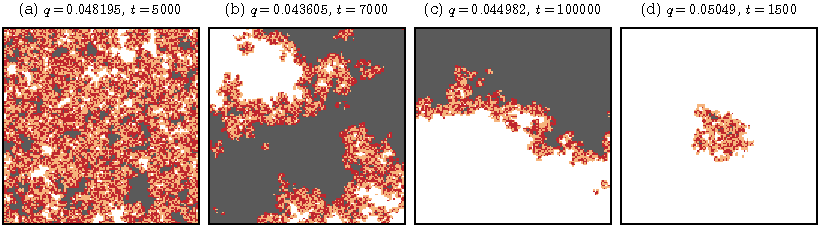
\includegraphics[width=\textwidth]{figs/fig_snap}
\caption{Configurations at $p = \alpha = 1/2$. Sites without a disagreeing Moore
neighbor are white (dead) or gray (alive); sites with at least one are orange (dead) or red
(alive). (a) The active phase, $q = 0.048195$, $t = 5000$, $L = 256$. (b) Decay of the metastable
active phase by nucleation and growth of the two absorbing phases, $q = 0.043605$, $t = 7000$
($256^2$ window of $L = 512$). (c) A wall between the two absorbing phases, wetted by a layer of the
active phase, $q = 0.044982$, $t = 10^5$. (d) A supercritical droplet, $q = 0.05049$, $t = 1500$,
grown from a disordered disk of radius 20.}
\label{fig:snap}
\end{figure*}

\subsection{Exactly two absorbing states}
\label{sec:lemma}

A configuration is absorbing when no site can flip, i.e., when $w(j_i) = 0$ for all $i$.

\textit{Lemma.} On the square lattice with the Moore neighborhood, every rule with $w(0)=0$ and $w(j)>0$ for
all $j\in\{3,\dots,8\}$ has exactly two absorbing configurations, the two uniform ones,
whatever the values of $w(1)$ and $w(2)$.

\textit{Proof.} A nonuniform configuration contains two nearest neighbors $x$ and $y$ (sharing an
edge) in different states. They disagree with each other, and they share four further Moore
neighbors, each of which disagrees with exactly one of them. Hence $j_x + j_y \ge 2 + 4 = 6$, so
$j_x\ge 3$ or $j_y\ge 3$, and that site flips with positive probability. $\square$

For $p>0$, Eq.~\eqref{eq:rule} gives $w(j)\ge pj/8>0$ for every $j\ge 1$, so the lemma applies.
For $0<p<1$ and $0<\alpha<1$ in the parameter range studied, $w(j)<1$ as well. Every configuration of a finite lattice then reaches consensus with
positive probability (by repeatedly flipping only the boundary sites of the live clusters), so
the two uniform states are the only recurrent ones.
At $p = 0$ the lemma fails only through $w(4) = w(5) = 0$, and it fails badly: every
configuration in which all sites have $j\in\{0,1,4,5\}$ is frozen. These include the two
checkerboards and the diagonal stripe patterns of width two, and their number grows
exponentially with the area (Appendix~\ref{app:frozen}). They were not observed as final states of the random-start simulations at $q>0$, and prepared patterns were typically destroyed by a single defect (Appendix~\ref{app:frozen}). Still,
they make ``two absorbing states'' false at $p = 0$. We retain that point only
as a directly simulated reference outside the exactly-two-state regime.
Appendix~\ref{app:frozen} also tests a direct regularization of the $p = 0$
rule, with a small flip probability $\epsilon$ at $j\in\{1,4,5\}$.
The measured front crossings suggest a smooth small-$\epsilon$ continuation;
they do not establish the infinite-time $p\to0^+$ limit.

\subsection{Monotonicity and mean-field theory}
\label{sec:mf}

The model is attractive (monotone) when $w(j)$ is nondecreasing in $j$ and $w(j)+w(8-j)\le 1$,
because a site's probability of being alive after an update then increases with the set of live
sites. The second condition holds for $q\le(1-\alpha)(1-p)$.
The first requires both $(1-p)\alpha\le p/8$, from $j=3\to4$,
and $q\le(1-p)\alpha+p/8$, from $j=2\to3$.
Thus, at $\alpha=1/2$ and in the tested range
$q\le(1-p)/2$, the model is nonmonotone for $p<0.8$ and monotone
for $p\ge0.8$. These conditions do not cover the $\alpha=1$ checks.
None of our arguments uses monotonicity. Finite-time front and seed signatures
also occur in the monotone region; the strongest coexistence evidence below
is at the nonmonotone value $p=1/2$.
Monotone nonlinear voter models with two absorbing states and an
active phase in two dimensions are known, the threshold voter
models~\cite{liggett1994}; what is at issue here is the order of the transition, not the
existence of an active phase.

At the level of a pair approximation on the Bethe lattice with $z = 8$ (Appendix~\ref{app:pa}),
the absorbing states are linearly stable for every $p<1$ and the disordered active state is
stable as well over the parameter range checked. The approximation is bistable
throughout that range and does not single
out a transition point: in a spatial system the phase is selected by which phase invades the
other. Mean-field bistability is precisely the situation in which washout is expected in two
dimensions~\cite{castellano2009}. Whether the two-dimensional transition is discontinuous is
therefore a question about fronts and fluctuations, and it is the question the simulations
address.

\subsection{Observables}

We measure the density $\rho$ of disagreeing nearest-neighbor bonds (the interface density per
bond), the fraction $\iota$ of sites with at least one disagreeing Moore neighbor, and the
magnetization $m = 2n-1$, where $n$ is the fraction of live sites. In the active phase
$\rho\approx 0.2$--$0.4$ and $m$ fluctuates around zero; in either uniform
absorbing phase $\rho = \iota = 0$.
The interface density is the order parameter. A transition is \emph{first order} in the sense
used here if (i) $\rho$ in the active phase stays finite as $q\to\qs{}^+$, independently of
system size, and (ii) the transition shows phase coexistence: a planar front between the active
phase and an absorbing phase is stationary at $\qs$ and moves with a velocity that changes sign
there, the active phase is metastable below $\qs$, and the probability
that an active droplet above $\qs$ reaches a macroscopic scale increases across
a characteristic finite radius.
At a GV point, instead, $\rho$ decays as $1/\ln t$ at
$q_c$; at a DP absorption transition it vanishes continuously. An Ising transition between two active phases instead concerns the magnetization and need not make $\rho$ vanish.

Spatial correlations use $s_i=2\sigma_i-1$ and the axis average
\begin{equation}
C(r)=\frac{1}{2L^2}\left\langle\sum_i s_i
\bigl(s_{i+r\hat x}+s_{i+r\hat y}\bigr)\right\rangle.
\label{eq:correlation}
\end{equation}
The random-start ensemble is exactly spin symmetric, so $\langle s_i\rangle=0$.
We retain the raw spin product, including $C(r)=1$ in absorbed configurations,
and do not subtract a separately estimated mean from each realization.

%=====================================================================================
\section{Methods}
\label{sec:methods}

\textit{Simulation.} We use a bit-parallel implementation in which each 64-bit word holds 64
sites and the neighbor counts and flip decisions are computed with bitwise operations. Each site
draws one uniform random number per step and flips if it is below the flip probability of its
class $(\sigma_i, j_i)$; all classes of a word share one bit-serial comparison, so the cost does
not depend on the number of distinct flip probabilities. Random numbers come from the
counter-based Philox$4\times 32$-10 generator~\cite{salmon2011}, keyed by the run's seed and
indexed by (time, row, word), so every run is bit-for-bit reproducible independently of the
number of threads and of restarts from checkpoints. The code passes a bit-exact comparison with a
naive per-site implementation for several rules and lattice shapes, and statistical tests of
the per-class flip frequencies (Appendix~\ref{app:numerics}). Near the transition it performs
about $10^9$ site updates per second per core. The extended dense-lattice
campaign uses a CUDA backend built from the same integer update and random-number
functions. CPU and GPU outputs agree bit for bit in the validation cases,
including large lattices, directed profiles, and checkpoints transferred in
both directions (Appendix~\ref{app:numerics}).

\textit{Protocols.} We use five kinds of runs.
(i) \emph{Bulk}: random initial condition with density $1/2$ on an $L\times L$ torus.
(ii) \emph{Strip fronts}: on an $L_x\times L_y$ torus, the rows $y<L_y/2$ start random and the
rest dead, giving two flat fronts between the active phase and the absorbing state. The per-row
interface counts are recorded, each front is located at a fixed fraction of
the relaxed interior activity, and the velocity $v$ is half the slope of the
strip width, $W(t) = W_0 + 2vt$,
fitted while the geometry remains a separated pair of fronts. The reference
level and validity windows are specified in Appendix~\ref{app:numerics}.
(iii) \emph{Tilted bands}: a band of direction $(a,b)$, the sites with
$(a y - b x)\bmod L < L/2$, on an $L\times L$ torus. Its two edges have total length
$2L\sqrt{a^2+b^2}$. Profiles binned along the normal locate both edges directly;
their separation gives the normal velocity without converting total activity
into an area.
(iv) \emph{Droplets and seeds}: a disk of radius $R$ whose sites are alive with probability $1/2$
(or a $2\times 2$ block of live sites) in the all-dead state. Many independent replicas are run;
since a site with $j = 0$ never flips, only the bounding box of the active region needs to be
updated, which is exact and makes each replica cheap. A replica stops when it
dies, reaches the lattice edge, or reaches its declared time horizon.
For the droplet experiment, $P_{\rm grow}$ is the probability of reaching
the edge before extinction and before that horizon. In seed-survival curves,
escaped replicas are retained as a separately recorded contribution; they
bound rather than directly measure survival after escape.
(v) \emph{Walls}: all-alive rows $y<L_y/2$ and all-dead rows above, i.e., two flat walls between
the two absorbing phases and no active phase at $t = 0$.
Times are in steps (one synchronous update of all sites). Error bars are standard errors over
independent runs unless stated otherwise.

\textit{Statistical analysis.} The reanalyzed flagship bulk data and the new
fixed-manifest campaigns use every run in complete, predetermined seed groups,
with no density filter or conditioning on survival. Supporting parameter surveys
retain their separately stated windows and selection protocols.
A partially finished fixed group is retained for diagnostics but not
used as an unconditional ensemble: absorption can make a run finish sooner
than a surviving trajectory. We integrate each sampled
trajectory in time before averaging independent runs; a trajectory is extended
by its known constant state after absorption. The half-density time is the first
recorded crossing of $\rho<0.145$ after $t=10^3$, half a reference density
$\rho_{\rm ref}=0.29$ near the flagship transition. It is distinct from complete
consensus. Five legacy $L=64$ runs already below this threshold at the analysis
origin are marked left censored at $10^3$, with lower bound zero. Other
first observed crossings retain the preceding output time as a recording-grid
diagnostic. Activity is not monotone, so brief unobserved dips can occur earlier;
these brackets are not rigorous bounds on its first physical passage.
Unobserved events are right censored, and survival curves and restricted mean times retain
that censoring. An event-free ensemble supplies right-censored observations
and a bound on finite-time survival, not a measured mean lifetime.
Independent-run resampling gives the reported bootstrap
intervals. For the four-run large-system groups these are approximate measures
of observed run variation and do not account for rare outcomes absent from
the sample. Event counts and systematic fitting-window checks are reported
separately.

%=====================================================================================
\section{The transition at $p = 1/2$}
\label{sec:flagship}

We first establish the discontinuity at $p = 1/2$, where bulk and interfacial
measurements give the best resolved coexistence tests. This point lies in the
nonmonotone part of the model, away from the voter limit. Figure~\ref{fig:snap} shows typical configurations.

\subsection{Fronts and their orientation}
\label{sec:fronts}

A strip of the active phase next to the absorbing state grows on one side of
the transition and shrinks on the other. The broad survey places reversal
near $q=0.04592$; the longer measurements below refine this location.
Behind a retreating front, the interior retains a substantial interface-site
fraction ($\iota_{\rm in}\simeq0.71$ at $q\simeq0.0436$, compared with about
0.76 near reversal). The active region is therefore invaded coherently before
it disappears. At a continuous transition the asymptotic active density would
instead vanish at the boundary. A finite-time retreating interface alone
does not distinguish these cases; we compare it with bulk and nucleation
measurements below. Front reversal also locates phase competition in the
four-species alliance model~\cite{szabo2004} and in spatial bistable
systems~\cite{durrett1994,durrett2009}.

In nonequilibrium systems, the reversal point can depend on front orientation.
Between the extreme crossings, a window of generic coexistence can open in
which sufficiently large droplets of either phase shrink by
faceting~\cite{toom1980,bennett1985,wang2015}. We compare bands with normals
$(1,0)$, $(2,1)$, and $(1,1)$, at $0^\circ$, $26.6^\circ$, and $45^\circ$
to the axes. Figure~\ref{fig:orient} shows the broad survey at $p=0.1$, $1/2$,
and $0.9$, with $L=4096$, eight seeds per point, and $T=2\times10^5$.
The outermost threshold crossings of the smoothed profile locate the band;
interior holes do not terminate this envelope. The smoothing length is nine
lattice spacings in the physical normal direction for every orientation.

At $p=1/2$, local interpolation between the two points bracketing reversal,
using $t\ge2\times10^4$, gives $q^*=0.045919$, 0.045911, and 0.045923 for
these three normals. Their conditional 95\% seed-bootstrap intervals are
$[0.045912,0.045927]$, $[0.045902,0.045921]$, and
$[0.045912,0.045933]$, respectively. Time windows, threshold levels, and fit
curvature are varied separately to assess systematic sensitivity. Several
straight-line fits across the entire sampled range have significant lack of
fit; their formal errors are not used as the full uncertainty of a crossing.
The broad survey finds only small orientation differences, but does not by
itself establish a unique orientation-independent transition point. It
constrains a broad generic-coexistence window of the type observed in
Ref.~\cite{wang2015} and motivates the finer comparisons below.

\begin{figure*}
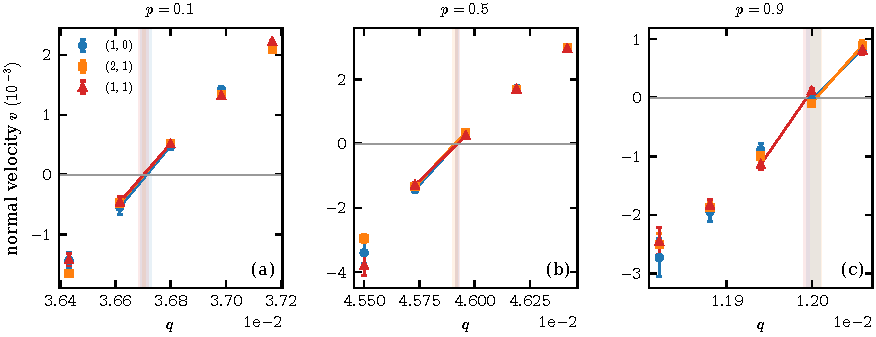
\includegraphics[width=\textwidth]{figs/fig_orient}
\caption{Normal velocity of a band of the active phase against the absorbing state, for normal
directions $(1,0)$, $(2,1)$, and $(1,1)$, at $p = 0.1$, $1/2$, and $0.9$; $L = 4096$, $T = 2\times10^5$,
eight seeds per point, velocity from the width of the band tracked along its normal for
$t\ge2\times10^4$. The horizontal coordinate is the actual probability $q$.
Lines interpolate the two seed-averaged velocities bracketing reversal;
shaded bands are conditional 95\% run-bootstrap intervals for the crossing.
Smoothing uses the same physical normal length for all orientations.
Farther below reversal the strip can nucleate absorbing domains internally,
so the broad-range velocity curve need not be linear.}
\label{fig:orient}
\end{figure*}

The fine-grid campaign extends these tests to $L=8192$ and 16384 and
$T=2\times10^6$ (Fig.~\ref{fig:gpu_fronts}). At $L=8192$, all five
probabilities and all three orientations have four completed independent
runs. Over $10^6\le t\le2\times10^6$, the local crossings are
0.0459387, 0.0459396, and 0.0459398 for normals $(1,0)$, $(2,1)$,
and $(1,1)$, respectively. Their spread is $1.0\times10^{-6}$, with a
conditional 95\% bootstrap upper value of $1.02\times10^{-5}$; simultaneous
pairwise intervals include zero. Varying the profile threshold from 0.2
to 0.5 gives crossings spanning 0.0459371--0.0459442 at this size and
window. At $L=16384$, the axial and tilted crossings differ by
$4.7\times10^{-6}$, with a simultaneous 95\% bootstrap interval
$[2.3,8.5]\times10^{-6}$. Thus a small direction dependence is resolved
at this finite observation time; its asymptotic extent remains open.
The shift relative to the short survey also shows why
observation time must enter the uncertainty assessment.

\begin{figure*}
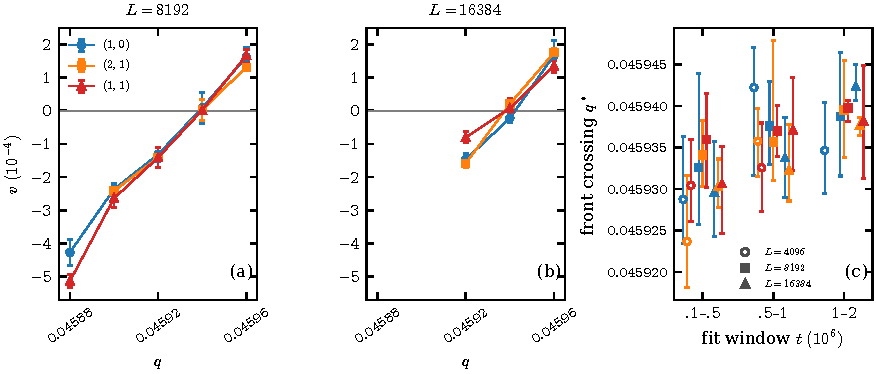
\includegraphics[width=\textwidth]{figs/fig_gpu_fronts}
\caption{Fine-grid front measurements at $p=\alpha=1/2$.
(a,b) Normal velocities at $L=8192$ and $16384$, fitted over
$10^6\le t\le2\times10^6$; four independent bands per point, and bars are
one standard error over runs. The profile threshold is 0.3 of the
reference activity at $t=10^3$. Colors and markers distinguish the three band
normals. Each included group retains a separated pair of fronts throughout
the stated fit window in every run.
(c) Local bracketing estimates of the velocity zero for three successive
windows; colors denote the same normals, while marker shapes denote $L$.
The $L=4096$ groups have eight runs, and the larger sizes four.
Intervals are conditional 95\% run-bootstrap intervals for each chosen
window and threshold. The variation between windows and orientations is
shown separately from sampling uncertainty.}
\label{fig:gpu_fronts}
\end{figure*}

Independent $L=8192$ cohorts followed to $5\times10^6$ steps test the
remaining time dependence (Fig.~\ref{fig:gpu_fronts5m}). For axial bands,
four new runs at each of $q=0.04593$, 0.04594, and 0.04595 give a crossing
of 0.0459340 over $2$--$3.5\times10^6$ and 0.0459435 over
$3.5$--$5\times10^6$. Resampling the same runs in the two windows gives
a paired shift of $9.4\times10^{-6}$ with a conditional 95\% interval
$[4.9,12.1]\times10^{-6}$. The change has the same sign at profile
thresholds 0.2 and 0.5. All fitted bands remain geometrically valid;
at $q=0.04594$, all four interiors retain more than 90\% of the reference
activity at the final time. This is
residual time dependence of an intact front, distinct from the fragmenting
near-voter strips discussed below. It enters the coexistence resolution
rather than being interpreted as demonstrated stationarity.
The local late-window crossings for the diagonal and tilted bands are
0.0459410 and 0.0459390. The diagonal paired change is not resolved.
For tilted bands, one $q=0.04595$ run exceeds the width cutoff at
$t=4.5\times10^6$ with threshold 0.3. The local root remains bracketed
by valid $q=0.04593$ and 0.04594 groups, but the predeclared whole-grid
paired contrast is withheld. At threshold 0.5 all three groups retain
valid geometry and the paired-shift interval includes zero.

\begin{figure*}
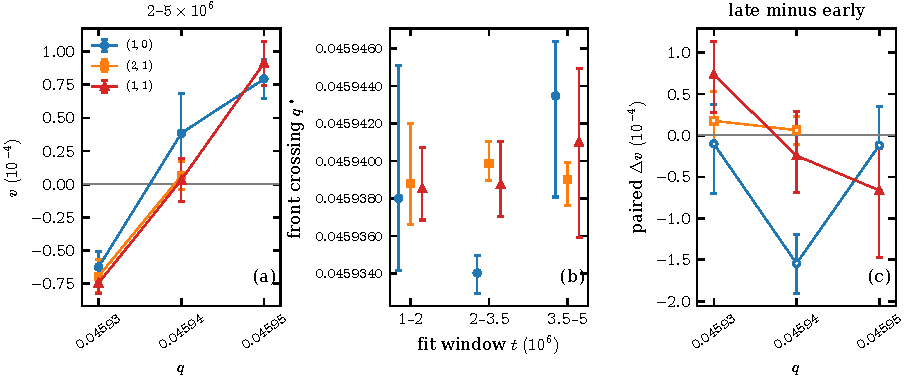
\includegraphics[width=\textwidth]{figs/fig_gpu_fronts5m}
\caption{Independent long-time front test at $p=\alpha=1/2$,
$L=8192$, with four new seeds per $(q,\mathrm{normal})$ and $T=5\times10^6$.
These cohorts are separate from the original $T=2\times10^6$ cohorts.
(a) Normal velocities fitted over $2$--$5\times10^6$, with one standard
error over runs. (b) Local bracketing crossings in successive windows
within the new cohorts, with conditional 95\% run-bootstrap intervals.
(c) Paired differences $v_{3.5\text{--}5\times10^6}-v_{2\text{--}3.5\times10^6}$;
each difference uses the same run in both windows, and bars are 95\%
run-bootstrap intervals. The profile threshold is 0.3. Only complete
predeclared four-seed groups with valid separated-front geometry throughout
both windows contribute. Threshold and interpolation choices remain
separate systematic uncertainties.}
\label{fig:gpu_fronts5m}
\end{figure*}

A further independent axial grid extends the same three probabilities to
$10^7$ steps, again with four new seeds per probability. All twelve runs
retain valid band geometry in both the $2$--$5\times10^6$ and
$5$--$10\times10^6$ windows at all three thresholds. At threshold 0.3,
the local crossing changes from 0.0459372 to 0.0459412; the paired shift
is $4.0\times10^{-6}$ with a conditional 95\% interval
$[2.4,5.6]\times10^{-6}$. The shift remains positive at thresholds 0.2
and 0.5, whose late crossings are 0.0459413 and 0.0459407. This independent
extension confirms residual front relaxation rather than demonstrating
stationarity. At $q=0.04594$, all four interiors retain more than 90\%
of their reference activity throughout the final window.

For common normalizations below, we adopt the rounded operational reference
$q^*=0.04594$ and vary it over $[0.04592,0.04596]$. This conservative
sensitivity range contains the available extended-front crossings and their
conditional intervals. It is not a pooled confidence interval or a bound
on the limiting coexistence point. The resolved time and orientation effects
remain part of the physical resolution of the study.

The direct test of generic coexistence is to place a large droplet of each phase in the
other~\cite{wang2015}: in a coexistence window both shrink. Figure~\ref{fig:drop2} shows, at
$p = 1/2$ and $L = 4096$, an active disk of radius 1000 in the dead state and a dead hole of the same
radius in the active state, at $q=0.0456842$, 0.0458221, 0.0460979,
and 0.0462358. At every sampled $q$ one of the two grows
while the other shrinks: above $\qs$ the active disk grows and the hole closes, below $\qs$ the
disk shrinks and the hole opens, at rates that follow the planar-front velocity corrected for
curvature, $\ds R/\ds t = \pm v - D/R$ (Sec.~\ref{sec:drops}). Disk mean
rates differ from this estimate by at most $2.1\times10^{-4}$ sites per step.
For holes the discrepancy is at most $3.0\times10^{-4}$ except at the lowest
$q$, where it reaches $6.1\times10^{-4}$: the surrounding metastable active
phase also begins to decay within the run (Sec.~\ref{sec:bulk}).
No interval in which both droplets shrink is resolved at these sampled
parameters. Together with the front measurements, this locates phase
competition in a narrow probability region. The droplet grid is too coarse
to resolve an orientation-dependent interval as small as the measured
front-crossing differences.

\begin{figure*}
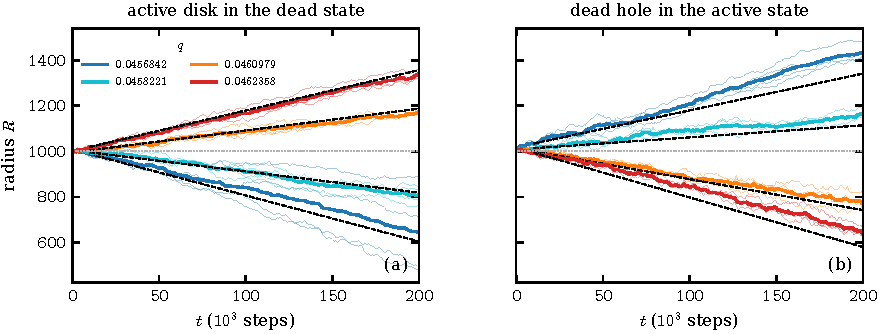
\includegraphics[width=\textwidth]{figs/fig_drop2}
\caption{Two-droplet test at $p = 1/2$ ($L = 4096$). Radius of (a) an active disk in the dead state
and (b) a dead hole in the active state, both of initial radius 1000; actual
$q$ values are given in the legend (thin lines: four seeds; thick lines:
their mean). Radii are obtained from the row profiles
(Appendix~\ref{app:numerics}). Dashed: $\ds R/\ds t = \pm v - D/R$,
with $v$ interpolated between the corrected seed-mean velocities of the
$(1,0)$ band of Fig.~\ref{fig:orient}(b) at each actual $q$, and $D = 0.20$
(Fig.~\ref{fig:drop}).}
\label{fig:drop2}
\end{figure*}

\subsection{Bulk: the jump and the metastable active phase}
\label{sec:bulk}

The extended campaign resolves finite bulk activity close to front
reversal on large systems and long observation windows (Fig.~\ref{fig:gpu_bulk}). At $q=0.04594$, all four $L=8192$
random-start runs remain active through $5\times10^6$ steps. Their
unconditional mean density over $2.5$--$5\times10^6$ is $0.28659$, with a
pointwise 95\% run-bootstrap interval $[0.28651,0.28667]$.
The difference between the second and first halves of this late window is
$7.2\times10^{-5}$, with interval $[-8.7\times10^{-5},1.6\times10^{-4}]$.
Thus no systematic late-window density decrease is resolved at this sampled
point; the spatial and front checks test its relation to coexistence separately.
Doubling the size to $L=16384$ gives a mean of 0.28661 at the same $q$
and time window. All twelve $L=16384$ runs at $q=0.04592$, 0.04594,
and 0.04596 remain active through $5\times10^6$ steps; none of the
three cohorts resolves a late-window density drift. The corresponding
means are 0.28498, 0.28661, and 0.28803. This comparison extends the
finite-density branch to substantially larger systems near front reversal.
At $q=0.04594$, the matched $2$--$5\times10^6$ window gives
$\chi_{8192}/\chi_{4096}=0.97$ with a pointwise 95\% run-bootstrap
interval $[0.84,1.08]$. The four independent runs at each size show no resolved
increase of this magnetic fluctuation scale upon doubling $L$.
The further doubling gives $\chi_{16384}/\chi_{8192}=0.95$ with interval
$[0.78,1.14]$ over the same window, again with no absorption in either
four-run cohort.

\begin{figure*}
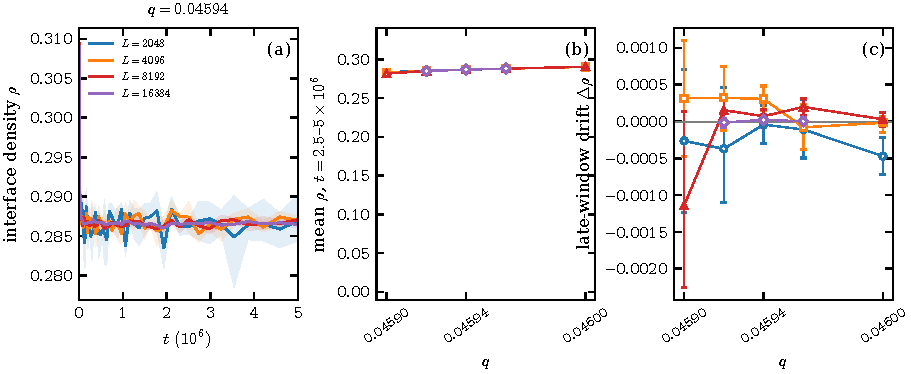
\includegraphics[width=\textwidth]{figs/fig_gpu_bulk}
\caption{Long, large-system bulk tests at $p=\alpha=1/2$, with four independent
random starts per $(L,q)$ and $T=5\times10^6$.
(a) Interface density at $q=0.04594$; bands are pointwise 95\% run-bootstrap
intervals. (b) Unconditional time-weighted density over
$2.5\times10^6\le t\le5\times10^6$ against the actual probability $q$.
(c) Difference between means over $3.75$--$5\times10^6$ and
$2.5$--$3.75\times10^6$; zero indicates no resolved drift between these
windows. Error bars in (b,c) are 95\% run-bootstrap intervals.
Every declared seed contributes; absorbed trajectories contribute their known
absorbing state for the rest of the observation window.}
\label{fig:gpu_bulk}
\end{figure*}

The final configurations provide a direct spatial check
(Fig.~\ref{fig:spatial_v2}). At $q=0.04594$, both $L=8192$ and 16384
give $C(128)\simeq0.0046$. For $L=16384$, $C(r)$ decreases from
0.427 at one lattice spacing to $5.7\times10^{-4}$ at $r=256$;
the pointwise intervals at $r=512$ and 1024 include zero. Signed
long-distance fluctuations are retained rather than clipped or fitted
to an assumed positive tail. The observed decay occurs on scales much
smaller than the box, complementing the density and magnetic-moment
comparisons. These are final-time measurements, not an extrapolation
of a correlation length to the transition.

\begin{figure*}
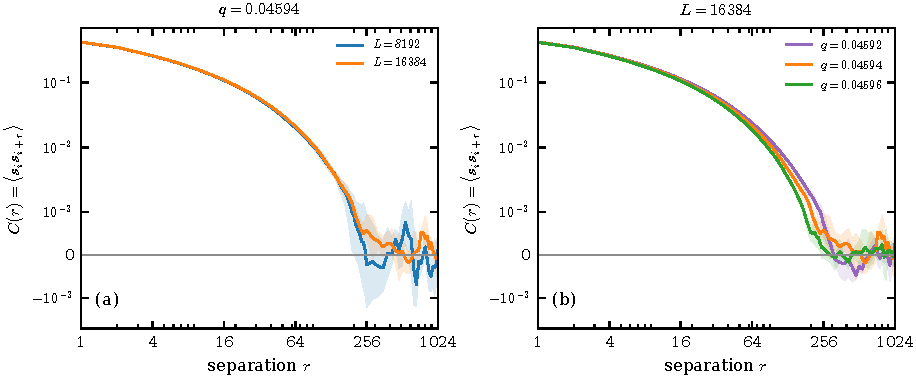
\includegraphics[width=\textwidth]{figs/fig_spatial_v2}
\caption{Direct spatial correlations at $p=\alpha=1/2$, measured in the
final configurations at $T=5\times10^6$, with four independent runs per
curve. The observable is the raw axis-averaged spin product in
Eq.~\eqref{eq:correlation}. (a) Size comparison at $q=0.04594$.
(b) Three probabilities at $L=16384$. Shading gives pointwise 95\%
run-bootstrap intervals; all declared configurations are included.
The vertical scale is logarithmic outside $|C|\le10^{-3}$ and linear
inside that interval, displaying both signs of the small long-distance
fluctuations. No functional form is fitted.}
\label{fig:spatial_v2}
\end{figure*}

Earlier bulk runs from random initial conditions (Fig.~\ref{fig:bulk}) give late-window
estimates of the active-phase interface density. At the points above $\qs$
shown in this survey, it settles within $10^3$--$10^4$ steps and then stays
constant to the end of the runs ($t = 2\times10^5$--$10^6$), independently of $L$ from 256 to 4096
within the run-to-run errors: $\rho = 0.3021$--$0.3023$ at $q = 0.046359$
and $0.3108$--$0.3113$ at $q=0.046818$
[Fig.~\ref{fig:bulk}(b)]. Even at $q = 0.0459$, the active phase
holds $\rho\simeq0.28$ for the full run ($10^6$ steps for $L\le 1024$, $3\times10^5$ and
$2\times10^5$ for $L = 2048$ and 4096) at every $L\ge 512$.
Such persistence can occur on the metastable side, so bulk persistence alone
does not locate the boundary. The finite-density branch persists to the
front-reversal region, supporting a discontinuity of order 0.28.
The magnetic second moment of the active phase,
$\chi_L = L^2\langle m^2\rangle$, grows toward the transition: its estimates are
$60$--$66$ at $q=0.05049$ and $305$--$463$ at $q=0.046359$ for $L=512$--4096.
At $q=0.0459$ they are of order $10^3$ for $L\ge1024$, with substantial
run-to-run uncertainty and no resolved growth with size. These data do not
show the increasing susceptibility expected at an Ising critical point.
Measured directly from stored configurations at $q=0.046359$ ($L = 2048$,
$t\ge 10^5$), the two-point function of the local spin $s_i=2\sigma_i-1$
falls to $0.40$ at one lattice spacing. Local exponential fits give
$\xi = 15$--$18$ over $4\le r\le 40$ and $10\le r\le 60$; at $q=0.05049$,
$\xi = 7$--$9$.

Below $\qs$ the active phase is metastable. At $q = 0.045441$ its density stays within 12\% of
the apparent active-branch plateau for $10^4$ steps and then collapses at an accelerating rate
[Fig.~\ref{fig:bulk}(a)]. The accelerating collapse and visible growth of absorbing
droplets [Fig.~\ref{fig:snap}(b)] support nucleation-driven decay.
Where droplets of opposite type meet, a layer of the active phase
remains between them (Sec.~\ref{sec:wall}), so $\rho$ does not drop to zero at once but to a slowly
coarsening network of wetted walls. The recorded half-density time $\tau$ grows steeply as
$q\to\qs$: $\tau = 3.4\times10^3$, $8.0\times10^3$, $1.6\times10^4$, $2.6\times10^4$, and
$7.0\times10^4$ at $q=0.04131$, 0.043605, 0.044523, 0.044982, and 0.045441.
It saturates at large $L$ [Fig.~\ref{fig:bulk}(c)]; at the closest of these points,
the means are $7.33$, $7.04$, $6.65$, and $6.70\times10^4$ for
$L=512$, 1024, 2048, and 4096. Many droplets nucleate independently, and the decay is a local
process (the multi-droplet regime of Ref.~\cite{rikvold1994}). Smaller systems ($L\le 128$) decay
sooner, because their size is only a few correlation lengths of the active phase, so that
the whole lattice can reach an absorbing state through one fluctuation.

\begin{figure*}
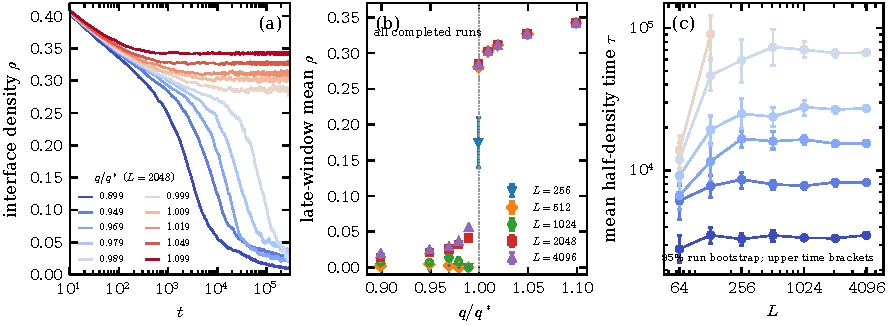
\includegraphics[width=\textwidth]{figs/fig_bulk05}
\caption{Bulk runs at $p = 1/2$ from random initial conditions ($\qs = 0.04594$). (a) Interface
density against time at $L = 2048$ for $q/\qs$ from 0.9 to 1.1 (one seed each).
(b) Time-weighted late-window density against $q/\qs$ for $L = 256$--4096,
using every completed run and all records over $t\ge T/2$ (2--16 runs per point).
Absorbed trajectories contribute zero after absorption; no activity filter is applied.
(c) Mean recorded half-density time below $\qs$ against $L$, shown only for
groups in which every trajectory crossed the threshold by the final time.
Times are first recorded crossings, including $10^3$ for five left-censored
$L=64$ runs; bars are 95\% run-bootstrap intervals, separate from output-cadence effects
(32 runs for $L\le
128$, 2--16 above; $T = 10^6$ for $L\le 1024$, $3\times10^5$ and $2\times10^5$ for $L = 2048$ and
4096).}
\label{fig:bulk}
\end{figure*}

The size dependence above $\qs$ is the opposite. Earlier $10^6$-step
cohorts at $q=0.046359$ had 32 of 32 consensus events at $L=64$, 25 of 32
at $L=128$, and none of 16 at $L=256$. We now test this stability signature
with independent, longer cohorts, keeping the two data sets separate.

A separate fixed ensemble extends the finite-size comparison at
$p=\alpha=1/2$, $q=0.046359$ to $T=10^7$ steps, with 32 independent
random starts at each of $L=64$, 128, 192, and 256
(Fig.~\ref{fig:lifetimes_v2}). The numbers reaching consensus are
32, 32, 6, and 0, respectively. The first recorded crossings of
$\rho<0.145$ are more frequent: 32, 32, 16, and 1.
Thus loss of half the reference activity and complete absorption are
separate observables. At $L=256$, the unconditional mean density over
$5\times10^6\le t\le10^7$ is 0.30230, with a 95\% run-bootstrap
interval $[0.30213,0.30246]$. With no consensus event among 32 $L=256$ runs,
the exact two-sided 95\% lower confidence limit for survival through
$10^7$ steps is 0.891. These observations extend the persistence window
and resolve strong size dependence; they do not determine an
asymptotic lifetime law.

The same contrast persists closer to coexistence. At $q=0.04605$, a
separate fixed ensemble follows 16 random starts at each of $L=192$,
256, and 384 to $3\times10^6$ steps. Consensus counts are 15, 6, and 0,
while recorded half-density events number 16, 6, and 1. The unconditional
mean densities over $1.5$--$3\times10^6$ are 0.060, 0.199, and 0.29235,
respectively. At $L=384$, the 95\% run-bootstrap density interval is
$[0.29100,0.29325]$,
and the exact two-sided 95\% lower confidence limit for survival through
the horizon is 0.794. Thus the size-dependent stability signature is
present at a second probability closer to the front-reversal region.

\begin{figure*}
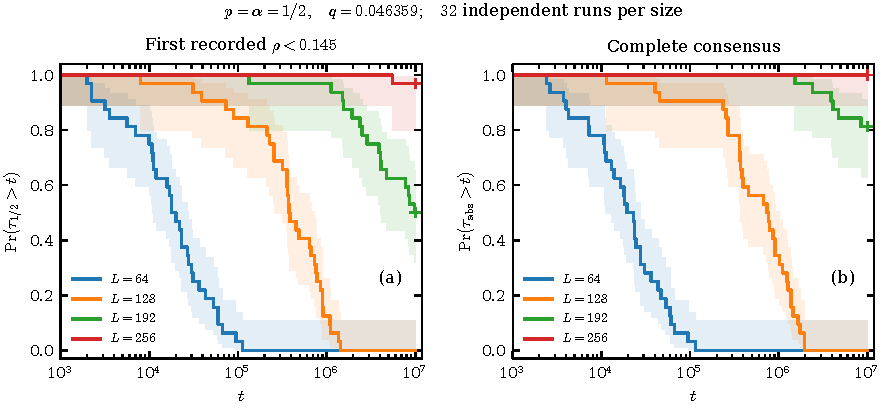
\includegraphics[width=\textwidth]{figs/fig_lifetimes_v2}
\caption{Long finite-size trajectories at $p=\alpha=1/2$, $q=0.046359$:
32 independent random starts per size, all followed until consensus or
$T=10^7$ steps. (a) Survival of the first recorded $\rho<0.145$ event,
searched at $t\ge10^3$ on the regular 1000-step and additional logarithmic
observation grid; recording-grid limitations are discussed in
Sec.~\ref{sec:methods}. (b) Survival to complete consensus.
Event counts for $L=64,128,192,256$ are $(32,32,16,1)$ in (a) and
$(32,32,6,0)$ in (b). Crosses denote right censoring. Shading gives
pointwise 95\% Kaplan--Meier bands (Greenwood log--log intervals away
from zero and one, with exact binomial edge bounds).}
\label{fig:lifetimes_v2}
\end{figure*}

In a multi-droplet description, the half-density time scales as
$\tau\propto(Iv^2)^{-1/3}$, where $I$ is the nucleation rate per unit area and
$v$ is the growth speed~\cite{rikvold1994}. The steep increase of $\tau$ on
approaching coexistence is consistent with slowing fronts and rarer nucleation.
Our finite interval of control parameters does not determine an asymptotic
nucleation law. In particular, a fit over these points cannot establish or
exclude the essential singularity expected from a classical nucleation barrier.

\subsection{Critical droplets}
\label{sec:drops}

Above $\qs$ the active phase is stable, but a small region of it usually disappears:
the probability of growth increases with its initial size. We placed a disordered disk of radius $R$
(sites alive with probability $1/2$) in the dead state and ran 500--1000 independent replicas per
$(q,R)$ until extinction, boundary escape, or the declared time horizon
(Fig.~\ref{fig:drop}). All replicas in the completed disordered-disk ensembles resolve
to extinction or escape. The macroscopic-growth probability $P_{\rm grow}$
rises from 0 to 1 over a factor of about 3 in $R$, and the radius at which it reaches
$1/2$ grows as $q\to\qs$: $R_c = 2.6$, 4.8, 7.9, 12.5, 21, and 42 at $q/\qs = 2.0$, 1.40,
1.20, 1.10, 1.05, and 1.02. Plotted against the inverse planar-front velocity at the same $q$,
$R_c$ is approximately linear [Fig.~\ref{fig:drop}(b)], $R_c\simeq D/v + \Delta R$ with $D = 0.207$ and an offset
$\Delta R = 1.4$ sites, consistent with relaxation of the random initial disk; equivalently,
$R_c v = 0.21$--$0.26$ over a factor of 11 in $v$. The deterministic growth
law $\ds R/\ds t = v-D/R$ has curvature radius $D/v$; the fitted initial
radius includes the offset $\Delta R$. Curvature slows a convex active
region. In this
description, linear front reversal predicts $R_c\propto1/(q-\qs)$ near
coexistence; the finite-time measurements support the relation to $1/v$ over
the sampled range. Joint resampling of the binomial droplet outcomes and
independent front runs gives a conditional 95\% interval $D\in[0.182,0.230]$;
changing the front threshold and fit start gives $D=0.199$--$0.212$.
A $2\times2$ block of live sites, the standard initial
condition of spreading experiments, is far below $R_c$: it reaches the boundary with probability
$0.042\pm0.003$ at $q = 1.4\,\qs$ and $0.20\pm0.01$ at $2\,\qs$, and with probability $0.011$ at
$1.2\,\qs$ and $0.003$ at $1.1\,\qs$ (4000 replicas each), although the active phase is the stable
one there; the $R = 0.75$ disks of Fig.~\ref{fig:drop}(a), $2\times2$ blocks in which each site is
alive with probability $1/2$, reach it with probability $0.014$ and $0.061$ at
$1.4\,\qs$ and $2\,\qs$.
Here $R_c$ is the radius at which $P_{\rm grow}=1/2$ for the specified box
and observation horizon, not a strict minimum size or an infinite-time
survival threshold. Smaller seeds have a nonzero chance to grow. The useful
nucleation diagnostic is the increase of this probabilistic radius and its
relation to the independently measured front velocity.

\begin{figure*}
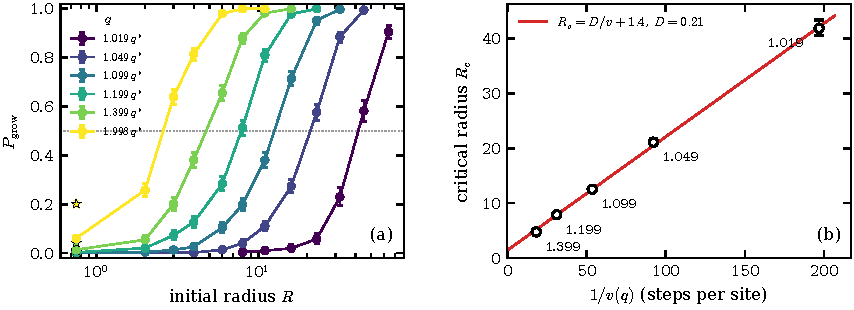
\includegraphics[width=\textwidth]{figs/fig_drop}
\caption{Critical droplets at $p = 1/2$. (a) Probability $P_{\rm grow}$ that a disordered disk of radius $R$
in the dead state reaches the lattice boundary before extinction and before
the declared time horizon, for $q/\qs$ from 1.02 to 2
(500--1000 replicas per point; at $R = 0.75$, a
$2\times2$ block with each site alive with probability $1/2$, 4000 replicas). Stars: the full
$2\times2$ block of live sites (4000 replicas). (b) Radius $R_c$ at
which $P_{\rm grow}=1/2$ against the inverse velocity of a planar front at the same $q$; labels
give $q/\qs$. The line is $R_c=D/v+\Delta R$. Disk protocols use
$L=512$--1024 and horizons $2\times10^4$--$3\times10^5$ depending on $q$;
the $2\times2$ block protocols use $L=1024$, $T=3\times10^4$.
Bars in (a) are 95\% binomial intervals from complete fixed-size replica
ensembles; vertical bars in (b) are conditional bootstrap intervals for the
interpolated $R_c$. The velocities use the corrected outer-envelope tracker.}
\label{fig:drop}
\end{figure*}

\subsection{Wetting of the wall between the absorbing phases}
\label{sec:wall}

A wall between all-alive and all-dead regions develops an active layer even when
the bulk active phase is metastable. Below the measured front reversal the
layer approaches a slowly varying thickness; above it the two edges move apart as active--absorbing
fronts. This geometry probes the competition among all three phases without
preparing an active region initially.

We measure the number $I=L_y\iota/2$ of interface sites per unit wall length and subtract
the $q=0$ value $I_0\simeq8.7$ to obtain the excess adsorption
$\Gamma=I-I_0$. Earlier measurements give an increase from about 10 at
$q=0.03672$ to about 109 at $q=0.0456705$. This increase is reproduced
across wall lengths $L_x=256$--4096 and transverse sizes $L_y=1024$--4096
(Fig.~\ref{fig:wall}). Runs last $10^6$--$3\times10^6$ steps.
For the late-window estimates we time-average each run over
$t\ge\max(3\times10^5,T/2)$ and then average independent runs.
Some walls wander far enough to consume one of the absorbing slabs. We terminate
their averaging windows before the live fraction leaves $[0.3,0.7]$, record
these truncations, and use the larger transverse boxes for the closest points.
The seven-point legacy fit below contains three truncated run windows and
omits one run with no usable window. Its two $L_y=4096$ points use the
available $L_y=1024$ baseline. The uncertainty of each shared $q=0$ baseline
is retained in the fit covariance; these legacy fits are conditional on the
stated geometry windows and baseline choices.

The increase of $\Gamma$ is robust, but a pure power law is sensitive to the
coexistence point and to corrections to scaling. With $q^*=0.04594$ and
$\delta=1-q/q^*$, fitting $\Gamma=A\delta^{-\psi}$ to the seven
$L_x=1024$, $L_y\ge2048$ points gives an effective $\psi=0.524$.
The fit is inadequate within the run-to-run errors: $\chi^2=74.7$ for five
degrees of freedom. The equally parameterized form
$\Gamma=A\delta^{-1/3}+B$ instead gives $A=20.28$, $B=-27.43$, and
$\chi^2=10.53$ for five degrees of freedom. Both fits minimize residuals in
adsorption units. Varying $q^*$ over $[0.04592,0.04596]$ moves the effective
pure-power slope from 0.506 to 0.541 and the offset-form $\chi^2$ from
3.74 to 27.03. An additive correction therefore changes the interpretation
of the apparent slope, while its fit quality remains reference dependent.
These legacy data do not establish an asymptotic exponent.

\begin{figure*}
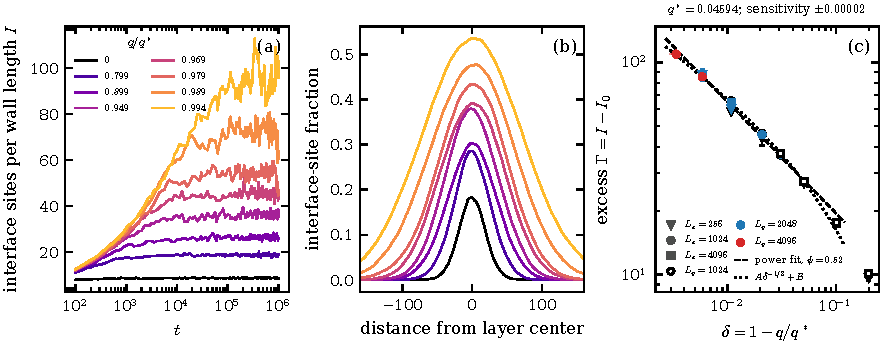
\includegraphics[width=\textwidth]{figs/fig_wall05}
\caption{Wetting at $p=1/2$, referenced to $q^*=0.04594$.
(a) Interface sites per unit wall length against time for $L_x=L_y=1024$
(four seeds per curve). (b) Interface-site fraction across the layer, centered
on its interface-weighted mean row before averaging late records.
(c) Excess adsorption for several box sizes (two to four seeds per point);
vertical bars show standard errors over runs including baseline uncertainty.
Horizontal bars on the fit points show the effect of varying $q^*$ by
$\pm0.00002$, a systematic sensitivity range. The dashed pure-power fit and
dotted $A\delta^{-1/3}+B$ fit use the same seven points with $L_x=1024$,
$L_y\ge2048$ and $\delta\le0.1$. The offset reduces the residuals, but neither fit determines the
asymptotic law.}
\label{fig:wall}
\end{figure*}

The extended test uses $L_y=8192$, wall lengths $L_x=4096$ and 16384,
and four independent $10^7$-step runs at each of three closer probabilities
(Fig.~\ref{fig:gpu_wetting}). Every ensemble is complete and retains the
full $5\times10^6$--$10^7$ averaging window, with a matched-size
$q=0$ baseline from two $2\times10^6$-step runs. All wall-separation
and global-density geometry checks pass. At $L_x=16384$, the excess
adsorptions are 133.27, 166.15, and 190.86 for $q=0.04584$, 0.04588,
and 0.04590. The corresponding $L_x=4096$ values are 134.80, 168.37,
and 199.90. At the closest probability, the larger system has about
4.5\% less adsorption; the run-bootstrap interval for this size difference
excludes zero. Its adsorption also declines by about 0.6\% between the
two halves of the late window, a small but resolved temporal change.
These data extend the observed thickening while exposing finite-size
and finite-time corrections.

The new points test predictions from the earlier fits. At each fixed
front-derived reference, both candidate forms are fitted only to the
seven legacy points; their parameter uncertainty and shared-baseline
covariance are propagated to the predictions. Agreement at one new
probability does not imply a joint description of all three. The
extended measurements show discrepancies beyond their sampling errors
from the legacy extrapolations, together with the size and time effects
above. The analysis therefore does not assign an asymptotic wetting
exponent or treat either two-parameter extrapolation as a converged law.

\begin{figure*}
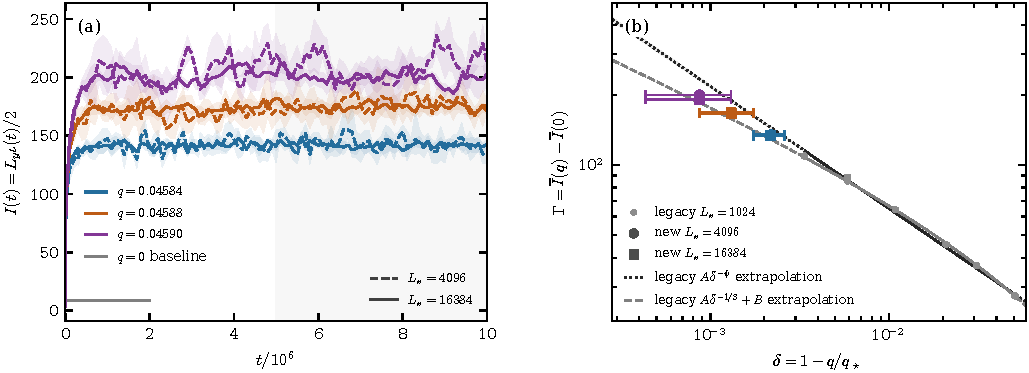
\includegraphics[width=\textwidth]{figs/fig_gpu_wetting}
\caption{Extended wall trajectories at $p=\alpha=1/2$, $L_y=8192$,
and $L_x=4096$ or 16384. Each nonzero-$q$ group contains four independent
runs to $10^7$ steps; each matching $q=0$ baseline contains two runs to
$2\times10^6$. (a) Interface sites per unit wall length. Line styles
distinguish $L_x$, and shading gives pointwise 95\% run-bootstrap
intervals. The gray span marks the $5$--$10\times10^6$ averaging window.
(b) Excess adsorption relative to the matched baseline. Vertical
intervals include shared-baseline sampling uncertainty; horizontal bars
show coexistence-reference sensitivity. Gray points and both
two-parameter fits use only the seven earlier $L_x=1024$ points.
Dashed and dotted continuations are predictions for the new data, with
conditional parameter-bootstrap bands at $q^*=0.04594$. These bands
exclude reference sensitivity and size/time systematics. No exponent is
fitted to the new data.}
\label{fig:gpu_wetting}
\end{figure*}

The observed layer thickening is consistent with complete wetting: near
coexistence an absorbing--absorbing interface separates into two
absorbing--active interfaces. Active boundary layers also occur between
defensive alliances~\cite{szabo2007}. In equilibrium, the interface between two
ordered phases can be wetted by the disordered phase at a first-order Potts
transition~\cite{selke1983,carlon1999}; fluctuating short-range interfaces in
two dimensions give the exponent $1/3$~\cite{lipowsky1983,fisher1984,carlon1999}.
Nonequilibrium wetting has also been studied with a bounded
Kardar--Parisi--Zhang interface~\cite{hinrichsen1997wet,munoz1998,delossantos2003}.
Here the layer is bounded by two fluctuating active--absorbing fronts.

The edges have short-distance roughness exponents close to $1/2$
(fits over $2\le r\le50$ give about 0.48--0.50 across the sampled
geometries), comparable to a free front, and the local thickness has a broad
distribution (Fig.~\ref{fig:rough}). These observations motivate a fluctuating
interface description but do not determine its large-distance interaction.
Larger wall lengths, smaller independently calibrated distances from
coexistence, and more seeds would be needed to test the asymptotic wetting law.

\begin{figure*}
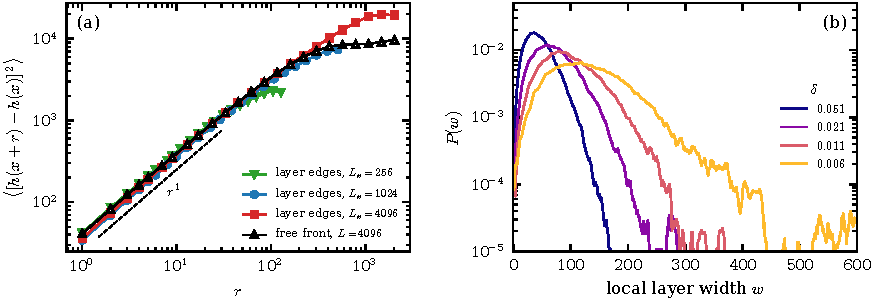
\includegraphics[width=\textwidth]{figs/fig_rough}
\caption{Edges of the wetting layer at $p = 1/2$, from configurations stored every $10^5$ steps for
$t\ge 10^5$ ($L_y = 2048$). (a) Height-difference correlation $\langle[h(x+r)-h(x)]^2\rangle$ of the
layer edges at $q=0.045441$ for $L_x = 256$, 1024, and 4096 (two to four seeds, both edges), and
of the two fronts of an active band near reversal, $q=0.04596$ ($L = 4096$, eight seeds, $4\times10^4\le
t\le 2\times10^5$); the dashed line is $\propto r$, i.e., $\zeta = 1/2$. (b) Distribution of the
local thickness $w$ of the layer (per column) at $L_x = 1024$ for
$q=0.043605$, 0.044982, 0.045441, and 0.0456705.}
\label{fig:rough}
\end{figure*}

%=====================================================================================
\section{The phase boundary toward the voter point}
\label{sec:line}

\subsection{Phase diagram}
\label{sec:phase}

Figure~\ref{fig:phase} shows the surveyed invasion boundary $\qs(p)$ from strip fronts at $\alpha = 1/2$,
together with the interface density of the active phase just above it. The line is nonmonotonic.
The directly simulated D\&N reference has $\qs(0)\approx0.0184$; the line
rises steeply at small positive $p$ (0.0207 already at $p = 0.01$)
to a maximum of $\approx 0.049$ near $p = 0.25$--$0.5$ and then approaches the voter
point approximately as $\qs\approx 0.25\,\alpha(1-p)$ over the sampled range
(Table~\ref{tab:line}). The initial rise is consistent with the voter
moves at $j = 4,5$, which D\&N forbids and which smooth interfaces.
The broad parameter survey finds sign-changing strip velocities and apparent
bulk plateaus $\rho_+ = 0.23$--$0.32$ at its stated observation times
[Fig.~\ref{fig:phase}(b)]. These finite-window densities do not determine the
limiting jump as $p\to1$. No tricritical point is resolved on this grid;
the longer-time assessment in Sec.~\ref{sec:voter} is essential near the endpoint.

\begin{table}
\caption{Broad finite-time survey at $\alpha=1/2$. Invasion thresholds
$\qs$ come from strip fronts (usually $L_x=2048$, $L_y=4096$, $T=10^5$,
2--4 seeds; $p=0$: five runs per probability across $L_x=2048,8192$;
$p\ge0.99$: note $b$), except for the refined $p=1/2$
estimate in Sec.~\ref{sec:fronts}. The bulk column gives the actual probability
$q_\rho$ and apparent plateau density $\rho_+$, using all selected runs at
$L\ge2048$ and time integration per run ($T\ge10^5$;
$p\ge0.98$: $T=10^6$--$1.5\times10^6$).
$c=\qs/[\alpha(1-p)]$. These densities are finite-window measurements.}
\label{tab:line}
\begin{ruledtabular}
\begin{tabular}{lllll}
$p$ & $\qs$ & $q_\rho$ & $\rho_+$ & $c$ \\
\hline
$0^{\,a}$ & 0.01837 & 0.0185 & 0.226 & -- \\
0.01 & 0.02070 & 0.021 & 0.245 & 0.042 \\
0.02 & 0.02280 & 0.02332 & 0.256 & 0.047 \\
0.05 & 0.02874 & 0.029 & 0.257 & 0.061 \\
0.1 & 0.03680 & 0.037904 & 0.288 & 0.082 \\
0.25 & 0.04932 & 0.05047 & 0.307 & 0.132 \\
0.5 & 0.04594 & 0.046359 & 0.302 & 0.184 \\
0.75 & 0.0276 & 0.0286 & 0.316 & 0.221 \\
0.9 & 0.01194 & 0.0122 & 0.290 & 0.239 \\
0.95 & 0.00619 & 0.0065 & 0.289 & 0.248 \\
0.98 & 0.00252 & 0.0025704 & 0.260 & 0.252 \\
0.99$^{\,b}$ & 0.00128 & 0.00128$^{b}$ & 0.241 & 0.256 \\
0.995$^{\,b}$ & 0.00064 & 0.00064$^{b}$ & 0.234 & 0.256 \\
\end{tabular}
\end{ruledtabular}
\begin{flushleft}\footnotesize
$^{a}$Direct $p=0$ reference, where the model has additional frozen configurations
(Appendix~\ref{app:frozen}).\\
$^{b}$Runs of $1.2\times10^6$ ($p = 0.99$) and $1.6\times10^6$ steps ($p = 0.995$), four times the
crossover time $t_\times$ of Sec.~\ref{sec:voter}, four seeds, velocities fitted for $t\ge t_\times$
from the strip profile (Appendix~\ref{app:numerics}); from runs of $10^5$ steps the
crossing at $p = 0.995$ is 0.00062 (Sec.~\ref{sec:voter}).
The bulk averages combine the nearby probabilities 0.00128 and 0.0012827 at
$p=0.99$, and 0.00064 and 0.0006417 at $p=0.995$; these are descriptive
survey values, not a limiting-density extrapolation. Their pooled standard
errors describe variation across these nearby parameters and horizons.
The new $2\times10^7$-step runs at $p=0.995$, $q=0.000640$ show
continuing decay (Sec.~\ref{sec:voter}); the tabulated threshold and density
there are historical finite-window estimates.
\end{flushleft}
\end{table}

\begin{figure}
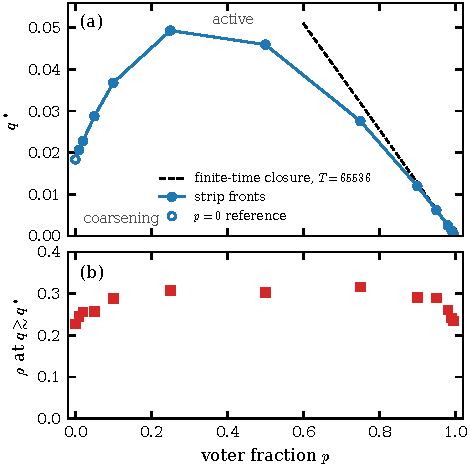
\includegraphics[width=\columnwidth]{figs/fig_phase}
\caption{(a) Finite-time invasion boundary $\qs(p)$ at $\alpha = 1/2$ from strip fronts (Table~\ref{tab:line}). Open
circle: the directly simulated $p=0$ reference with additional frozen states.
Dashed: the finite-time closure
$q_f(T)=c_f(T)\alpha(1-p)$ at $T=65536$, where $c_f=0.2553$;
this is a fixed-cutoff comparison, not an asymptotic prediction.
(b) Finite-time interface density near the earlier front estimates,
at points where a plateau was observed in the broad survey
($q_\rho$ in Table~\ref{tab:line}), with time integration per run and equal run
weights; bars are one standard error. Near-endpoint values require the longer-time
checks in Sec.~\ref{sec:voter}.}
\label{fig:phase}
\end{figure}

\subsection{Near the voter point}
\label{sec:voter}

As $p\to 1$ the transition approaches the voter point, where logarithmic corrections make every
diagnostic slow. A finite-window fit to one voter-model run at $L=4096$
gives $1/\rho\simeq0.184\ln t+2.13$ over $10^3\le t\le10^6$;
its slope depends on the fit start and is not an asymptotic amplitude.
A density that looks stationary over a finite window is therefore not enough.
We compare four complementary diagnostics at $p = 0.98$,
$0.99$, and $0.995$, with the noise strength measured by $\delta = q/\qs - 1$.

\textit{Bulk relaxation and front drift.} The earlier survey found apparent
plateaus $\rho\approx0.23$--$0.26$ over $10^6$--$1.5\times10^6$ steps at
$L=2048$ and 4096, including points very close to its estimated invasion
boundary. The sensitivity of that boundary to observation time already
signaled a long crossover. At $p=0.995$, a $10^5$-step strip estimate gives
$q\approx0.00062$, where the bulk subsequently decays; extending the strips
to $1.6\times10^6$ steps moves the crossing to approximately $0.000640$,
with a quoted spread of $5\times10^{-6}$ across the earlier estimates.
The analogous $1.2\times10^6$-step estimate at $p=0.99$ is about $0.00128$.
Table~\ref{tab:line} records this finite-time survey. Agreement between two
sizes over that horizon does not establish stationarity at longer times.
At $p=0.99$ the apparent plateau decreases on approaching the boundary:
$1/\rho$ changes from 3.60 at $q\approx1.19\,\qs$ to 4.11 near $\qs$.
These finite-window values alone distinguish neither a small limiting jump
nor logarithmically slow continuous vanishing.

The longer fixed ensembles at $p=0.995$ expose the limitation directly
(Fig.~\ref{fig:gpu_near}). At $L=4096$, the four-run mean density at
$q=0.000636$ falls from 0.201 over $10^6$--$2\times10^6$ steps to
0.027 over $5\times10^6$--$10^7$; all four runs reach consensus by
$10^7$. At $q=0.000640$, none reaches consensus by that time, but the
successive window means decrease from 0.228 to 0.216 to 0.207. At
$q=0.000644$ and 0.000648, the late means are 0.229 and 0.233 and no
late drift is resolved within the four-run uncertainty. These observations
separate collapse from persistence over a substantially longer horizon,
without identifying the limiting order parameter at the boundary.

Extending $L=8192$ runs to $2\times10^7$ steps makes the drift at
$q=0.000640$ clearer. The four-run mean falls from 0.189 over
$5\times10^6$--$10^7$ to 0.122 over $10^7$--$2\times10^7$,
with a 95\% run-bootstrap interval $[0.078,0.168]$ for the latter, and
one run reaches consensus. The difference between the second and first
halves of that window is $-0.055$, with interval $[-0.092,-0.027]$.
The earlier apparent plateau at this probability is therefore not a
stationary active-state measurement.
An independent midpoint ensemble at $q=0.000642$ retains activity in all
four runs, with late mean 0.2204 and interval $[0.2159,0.2231]$.
Its within-window drift is nevertheless resolved: $-0.0046$ with
interval $[-0.0077,-0.0015]$, about 2.1\% of its late mean.
At $q=0.000644$ and 0.000648, all four $L=8192$ runs remain active
through $2\times10^7$, with late means 0.2265 and 0.2326 and no resolved
drift within $10^7$--$2\times10^7$. This separates late decay from
persistence on the sampled grid; bulk persistence alone still does not
locate an asymptotic coexistence boundary.
Figure~\ref{fig:gpu_near20m} shows the full largest-system time traces
and their paired late-window changes.

The strip experiment has a related limitation. At $q=0.000640$, activity
within the initial strip interior decays strongly and only one of four
runs retains valid separated-front geometry throughout
$5\times10^6\le t\le10^7$. An envelope fitted to the fragmented band
would mix front motion with internal decay. We therefore do not assign
a stationary front velocity to that ensemble. At higher $q$ the interior
persists, but expanding bands can instead encounter the finite box.
Both failures are visible in the width and interior-activity diagnostics.

\begin{figure*}
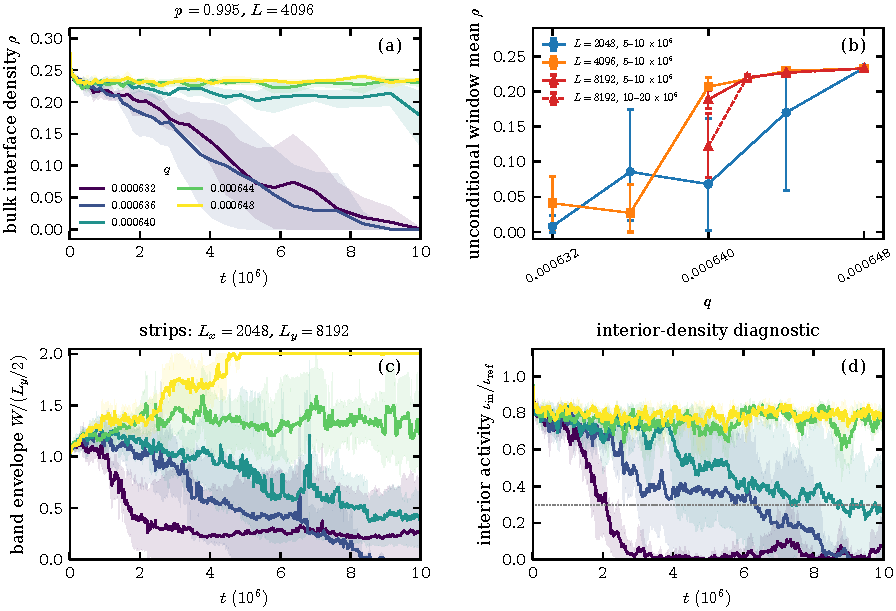
\includegraphics[width=\textwidth]{figs/fig_gpu_near}
\caption{Long-time tests near the voter point, $p=0.995$, $\alpha=1/2$;
four independent runs per parameter set. Colors in (a,c,d) denote the same $q$.
(a) Bulk density at $L=4096$ to $10^7$ steps.
(b) Unconditional time-weighted bulk means over the common
$5\times10^6\le t\le10^7$ window at three sizes, together with the later
$10^7$--$2\times10^7$ window at $L=8192$.
(c) Outer-envelope width of initially half-filled active strips,
$L_x=2048$, $L_y=8192$, normalized by the initial half-box width.
(d) Activity in the initial central interior region, relative to its
reference value at $t=10^3$. The dotted line is the profile threshold used
for the envelope. A changing interior density must be distinguished from
motion of a stationary front. Bands and bars are pointwise 95\%
run-bootstrap intervals. Absorbed trajectories are extended by their known
zero activity, and only complete predeclared seed ensembles are shown.}
\label{fig:gpu_near}
\end{figure*}

\begin{figure*}
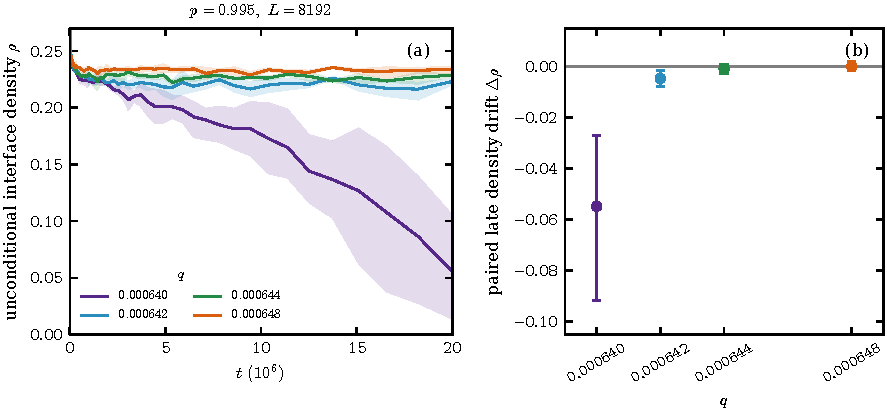
\includegraphics[width=\textwidth]{figs/fig_gpu_near20m}
\caption{Largest-system time dependence near the voter point, $p=0.995$,
$\alpha=1/2$, $L=8192$. All four predeclared independent runs at each actual
$q=0.000640$, 0.000642, 0.000644, and 0.000648 are followed to
$T=2\times10^7$. (a) Unconditional interface density; the trajectory absorbed
at $q=0.000640$ contributes zero for the rest of the horizon.
(b) Paired late drift, the time-weighted mean density over
$1.5\times10^7$--$2\times10^7$ minus that over
$10^7$--$1.5\times10^7$, computed within each run before averaging.
Bands and bars are pointwise 95\% empirical run-bootstrap percentile intervals,
enumerating all 256 ordered resamples of the four runs; their confidence
coverage remains approximate. The midpoint cohort at $q=0.000642$ was declared
independently after the original grid, and is not pooled with other cohorts.
A zero-containing drift interval does not establish stationarity.}
\label{fig:gpu_near20m}
\end{figure*}

\textit{Size dependence of the magnetic fluctuations.} A split into an Ising
and a DP transition would leave an ordered active window. At the Ising point,
$\chi_L=L^2\langle m^2\rangle\sim L^{7/4}$, giving
$\chi_{4096}/\chi_{2048}=2^{7/4}\simeq3.36$.
Unfiltered, time-weighted run estimates show much weaker size dependence
at several sampled active points [Fig.~\ref{fig:voter}(a)]. For example,
at $p=0.98$, $q=0.0025704$, the ratio is $1.09$ with a pointwise
95\% run-bootstrap interval $[0.82,1.52]$.
Closer to the endpoint and threshold the uncertainty is larger:
at $p=0.99$, $q=0.0012827$, the ratio is $0.92$ with interval
$[0.34,4.20]$, and at $p=0.995$, $q=0.000651$, it is $1.95$
with interval $[1.07,3.46]$. These latter intervals include the Ising
size factor; restricting both sizes to the common window
$2\times10^5\le t\le5\times10^5$ leaves similarly large uncertainty.
No ordered active interval is resolved by the present grid,
but these measurements cannot exclude a narrower interval near the boundary.
The new $p=0.995$ ensembles at $q=0.000648$ give
$\chi_{4096}/\chi_{2048}=1.18$ with interval $[0.72,1.98]$ over the
common $5\times10^6$--$10^7$ window; all four runs at each size remain
active. This constrains fluctuations at that sampled active point.
The further doubling gives $\chi_{8192}/\chi_{4096}=0.91$ with interval
$[0.48,1.70]$ over the same window, also without absorption.
Closer to the boundary, absorption in the smaller systems contributes
$m^2=1$ and prevents interpreting an unconditioned size ratio as an
equilibrium critical-scaling test.

\textit{Suppression of small seeds.} A $2\times2$ block of live sites in the dead state
spreads, in the voter model, with survival probability $P_s(t)\simeq A\ln t/t$~\cite{bramson1980},
i.e., a local exponent $\delta_{\rm eff} = -\ds\ln P_s/\ds\ln t$ approaching 1 from below. GV criticality has voter-like asymptotic spreading, but this does not impose a finite-time bound on $\delta_{\rm eff}$ in a nonlinear model~\cite{castellano2012,azizi2020}; at a DP point $\delta_{\rm eff}\to0.451$. Figure~\ref{fig:voter}(b)
shows $t\,P_s(t)$, which grows as $\ln t$ for the voter model. At sampled
nonlinear-model points where the bulk remains active over the observation
window, this quantity instead decreases over substantial intervals.
The contrast is consistent with a nucleation barrier to invasion from
small seeds. At $p=0.99$, $q=0.0012954$, an independent predeclared
ensemble of $8\times10^6$ seeds leaves 19 survivors and no escapes at
$t=10^6$. Thus $P_s=2.375\times10^{-6}$, with an exact two-sided 95\%
binomial interval $[1.430,3.709]\times10^{-6}$. All sixteen fixed-size
shards of 500000 replicas completed with adaptive stopping disabled.
Between $t_1=63096$ and $t_2=251189$, the survival count falls from
793 to 97. The approximately factor-four-window estimate
$\delta_{\rm eff}=-\ln[P_s(t_2)/P_s(t_1)]/\ln(t_2/t_1)$ is 1.52,
with a pointwise 95\% conditional-binomial interval $[1.39,1.66]$.
The decay slope does not keep increasing: the last supported factor-four
window, $t=223872$--891251, gives 1.26 with interval $[0.99,1.59]$.
No terminal slope is quoted because 19 survivors fall below the
predeclared minimum count of 20. Overlapping windows are correlated
and are not fitted as independent exponent estimates. These observations
quantify intermediate-time seed suppression while leaving the asymptotic
survival probability and critical scaling unresolved.
At $p=0.995$, $q=0.0006324$, below the estimated threshold, none of
$3\times10^6$ seeds survives to $10^6$. Further above threshold the seeds
overshoot and then level off: at $p=0.99$, $q=0.0013335$, running to
$t=10^6$ on $L=8192$ gives 40 recorded survivors or escapes, compared with
88 at $10^5$. One of the terminal replicas has escaped, so the observed
late-retention ratio is bounded by $39/88$ and $40/88$, approximately
$0.44$--$0.45$, before sampling uncertainty; the voter asymptote gives
about 0.12. These higher-$q$ shards stopped at survivor targets, with
750839 replicas in total. Their curves are descriptive finite-time
evidence of slower late decay, and neither their stopping protocol nor
their observation horizon identifies a limiting survival probability.

\textit{Walls are wetted below the threshold.} A flat wall between the two absorbing phases
(protocol v) roughens like a voter interface at first, $W\propto t^{1/2}$, independent of $q$. After
a crossover time $t_\times$, $q$ takes over (Fig.~\ref{fig:voter}(c)). Below $\qs$ ($\delta =
-0.02$ at $p\le 0.98$, $-0.03$ at $0.99$, $-0.05$ at $0.995$) the wall turns into a slab of the
active phase with a long-lived finite width, $W(10^6)\approx 200$,
450, 670, and 820 for $p = 0.9$, 0.98, 0.99, 0.995, whose interior has an interface-site
fraction of 0.46--0.51, comparable to the earlier finite-window bulk estimates
near reversal (0.47--0.58); the pure voter wall
keeps widening. Above
$\qs$ the slab edges move outward at the strip-front velocities.
The crossover time increases from $\approx10^4$ at $p=0.9$ to
$\approx4\times10^5$ at $p=0.995$; the sampled-range fit
$t_\times\propto(1-p)^{-1.3}$ is an effective description, not an
asymptotic scaling law. This initial crossover marks the time at which
the perturbation becomes visible. The new longer runs show that it need
not mark final relaxation: the transition order remains unresolved at
$p=0.995$ and closer to the voter point.

These measurements follow the invasion boundary toward the voter point
and provide supporting evidence for a continuation of discontinuous behavior.
They do not establish that continuation at $p=0.995$, where threshold
uncertainty and relaxation times are largest. Accelerated seed extinction
supports a nucleation interpretation, rather than a universal finite-time
test excluding GV criticality. We distinguish these endpoint results from
the well-resolved coexistence at $p=1/2$ and from a claim about every fixed
$p<1$.

\begin{figure*}
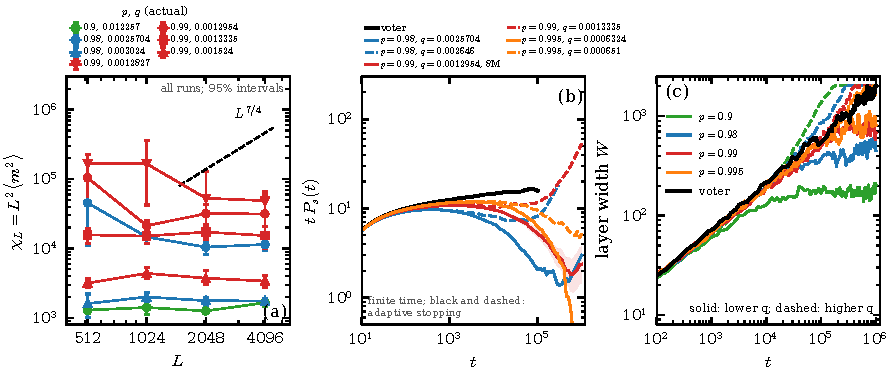
\includegraphics[width=\textwidth]{figs/fig_voter}
\caption{Near the voter point. (a) Unconditioned magnetic second moment
$\chi_L = L^2\langle m^2\rangle$ from random starts for $p=0.9$, 0.98,
and 0.99; the legend gives actual $q$. Each point averages 2--8 independent
runs after time integration over $t\ge2\times10^5$, with final times
$5\times10^5$ or $10^6$. Bars are pointwise 95\% run-bootstrap intervals.
No activity filter is applied: trajectories reaching consensus contribute
$m^2=1$ thereafter, which affects the small systems. The dashed line is
the Ising law $L^{7/4}$. (b) Survival of a $2\times2$ seed in
the dead state, $t\,P_s(t)$, which grows as $\ln t$ for the voter model (black, $L = 2048$), decays
when small seeds are strongly suppressed, and would grow linearly for a
positive limiting survival probability. The red solid curve at $p=0.99$,
$q=0.0012954$ uses the complete independent fixed-$N$ ensemble of
$8\times10^6$ replicas. Shading gives pointwise 95\% binomial intervals
(Clopper--Pearson for sparse counts, Wilson otherwise). Other nonlinear
solid curves retain the earlier $3\times10^6$-replica ensembles.
The black voter reference and higher-$q$ dashed curves use adaptive
survivor-target stopping and are shown descriptively.
The black reference stops at 300 retained replicas out of 1,905,766,
including 11 escapes at $t=10^5$; its plotted retained fraction is the upper
survival bound. Lattice size is
$L=8192$ for the nonlinear models; escapes are recorded separately.
(c) Width $W$ of the active
layer on a flat wall between the two absorbing phases, $L_x=1024$, $L_y=4096$,
two seeds. The pairs of lower (solid) and higher (dashed) probabilities are
$(0.011662,0.012495)$, $(0.0024696,0.002646)$,
$(0.0012446,0.0013335)$, and $(0.0006076,0.000651)$ for
$p=0.9$, 0.98, 0.99, and 0.995, respectively. Black: the voter model
($p=1$, $q=0$).}
\label{fig:voter}
\end{figure*}

\subsection{Synchronicity and asynchronous updating}
\label{sec:async}

The D\&N weight $\alpha$ sets the scale of $\qs$. Near the voter point the measured threshold is consistent with proportionality to $\alpha$: strip fronts at $\alpha = 1/4$, $1/2$, and 1 for $p = 0.98$ and 0.99 give
$\qs\propto\alpha^{\beta}$ with $\beta = 1.00\pm0.02$ and $c = \qs/[\alpha(1-p)] = 0.248$--$0.258$
(Table~\ref{tab:alpha}), consistent with the finite-time closure of
Sec.~\ref{sec:theory}. At the directly simulated $p=0$ reference, the
finite-density branch persists at the sampled $\alpha$ values between $1/8$
and 1, with no tricritical point resolved on that grid.

To test sensitivity to parallel updating, we make the dynamics lazy: each site
is updated with probability $r$ per step (the flip table is multiplied
by $r$), so $r\to 0$ is continuous time and $rt$ is the physical time. At $p = 0.98$ the front
velocity still changes sign. Nominal linear fits give
$\qs(r)/\qs(1) = 0.864\pm0.010$, $0.858\pm0.016$,
and $0.870\pm0.012$ for $r = 1/2$, $1/4$, and $1/8$.
These legacy fits use selected profile windows and extrapolate slightly
beyond their fitted probability range. Alternative documented fit ranges
shift the ratios by as much as 0.05, beyond the quoted sampling errors.
No monotonic change among the sampled $r\le1/2$ is resolved within that
systematic variation. At
$p = 0.99$, $r = 1/4$, fronts just above $\qs(r)$ retreat for $\sim 10^5$ physical time units
before advancing, and the late-time crossing, $0.85$--$0.88$, agrees with $p = 0.98$. At the
representative point $p=1/2$, corrected outer-envelope tracking of three
strips over physical times $2.5\times10^4$--$5\times10^4$ gives a
finite-window crossing $q^*(1/4)\simeq0.03963$, or roughly 0.86 of the
synchronous value. Earlier windows and profile thresholds produce shifts
of several $10^{-3}$ in this ratio, so greater asymptotic precision is
not assigned. The bulk active phase at $q=0.040392$ has a late-window mean
$\rho\simeq0.2105$ through physical time $10^5$, while at $q=0.039474$
it decays slowly. Supporting near-voter runs show bulk plateaus over a
factor 40 in time at roughly 10\% above the nominal crossing, early seed
decay with $\delta_{\rm eff}>1$, and active wall layers below the nominal
crossing while the lazy-voter wall keeps widening. The legacy seed curves
use adaptive stopping, and boundary escapes contaminate their late retained
counts, so no survival plateau is inferred from them.
These finite-$r$ checks show robustness to reduced update probabilities.
Establishing the strict continuous-time transition requires an extrapolation
in $r$.

\begin{table}
\caption{Synchronicity and asynchrony near the voter point. Top: $\qs\propto\alpha$ (strip
fronts, four seeds; errors are seed bootstrap, systematic $\approx\pm2\%$). Bottom: lazy updating
with probability $r$ per step at $p = 0.98$ and $1/2$; $c(r)$ from simulation and, near the voter
point, from the theory of Sec.~\ref{sec:theory}. The $p=0.98$ bottom entries
are nominal finite-window, profile-selected estimates; parentheses give
sampling errors, while probability-fit-range changes shift their ratios
by up to 0.05. The $p=1/2$ entry uses the corrected envelope over physical
times $2.5\times10^4$--$5\times10^4$ and is rounded to reflect window and
threshold sensitivity. Theory entries use fixed dual time $T=65536$
for synchronous walks and physical dual time $rT=65536$ for lazy walks;
their parentheses include walk-sampling uncertainty only.}
\label{tab:alpha}
\begin{ruledtabular}
\begin{tabular}{lllll}
$p$ & $\alpha$ & $\qs$ & $c$ (sim.) & $c$ (theory) \\
\hline
0.98 & 0.25 & 0.001274(9) & 0.255 & \\
0.98 & 0.5 & 0.002515(19) & 0.252 & \\
0.98 & 1 & 0.005074(30) & 0.254 & 0.255(2) \\
0.99 & 0.25 & 0.000621(18) & 0.248 & \\
0.99 & 0.5 & 0.001292(7) & 0.258 & \\
0.99 & 1 & 0.002553(9) & 0.255 & \\
\hline
$p$ & $r$ & $\qs(r)/\qs(1)$ & $c(r)$ (sim.) & $c(r)$ (theory) \\
\hline
0.98 & 1/2 & 0.864(10) & 0.218 & 0.221(3) \\
0.98 & 1/4 & 0.858(16) & 0.216 & 0.206(4) \\
0.98 & 1/8 & 0.870(12) & 0.219 & 0.200(4) \\
0.5 & 1/4 & $\approx0.86$ & 0.159 & -- \\
\end{tabular}
\end{ruledtabular}
\end{table}

%=====================================================================================
\section{A finite-time voter closure near the voter point}
\label{sec:theory}

Near $p=1$, write $\varepsilon=1-p$ and $\kappa=q/\varepsilon$, so that
\begin{equation}
 w(j)=\frac j8+\varepsilon g(j),\qquad
 g(j)=\alpha R(j)-\frac j8+\kappa\delta_{j,2}.
 \label{eq:pert}
\end{equation}
Voter-model perturbation theory relates a weak microscopic perturbation to a reaction
term obtained by averaging over voter correlations~\cite{cox2013}. In $d\ge3$ the
required nontrivial voter equilibrium exists. In $d=2$ the voter model clusters and
that stationary reaction function is not defined~\cite{cox2025}. We therefore
separate an exact finite-time calculation from its use as a closure for the
perturbed model.

\subsection{Exact finite-time identities}

Start the unperturbed voter model from independent spins of mean density $u$, and
let $\langle\cdot\rangle_{u,T}$ denote its local law at time $T$. Define
\begin{equation}
 f_T(u)=\big\langle(1-2\sigma_0)g(j_0)\big\rangle_{u,T}.
 \label{eq:f}
\end{equation}
For this specified reference law, $f_T$ is exactly the mean density drift due to
the perturbation, divided by $\varepsilon$. It is not the drift evaluated in the
unknown stationary law of the perturbed process.

The reference expectation can be evaluated by voter duality. Nine coalescing walks
start at the origin and its eight Moore neighbors and run backward for $T$ steps.
For synchronous updating, distinct walks jump independently at each step and
coalesce when their new positions coincide. Each surviving lineage is assigned a
state independently, with probability $u$ of being live. This gives the polynomial
$f_T$ by summing over the lineage partitions and their colorings. We use the
recorded histograms of $10^6$ walk realizations at each cutoff.

Three identities substantially constrain the result. A perturbation linear in
$j$ gives zero drift. One- and two-lineage partitions also give zero by symmetry.
For a three-lineage partition, let $n_1,n_2$ be the numbers of neighbors in the
two classes not containing the origin. Its contribution is
\begin{equation}
 \begin{gathered}
 h(u)\,[g(n_1)+g(n_2)-g(n_1+n_2)],\\
 h(u)=u(1-u)(1-2u).
 \end{gathered}
 \label{eq:three}
\end{equation}
A four-lineage partition contributes the same cubic, with coefficient
$\sum_{i=1}^3g(n_i)-g(\sum_{i=1}^3 n_i)$.
Only partitions with at least five lineages can generate higher-degree terms.
In particular,
\begin{equation}
 f_T=\alpha f_{R,T}+\kappa f_{2,T}
 \label{eq:linearclosure}
\end{equation}
holds exactly at every fixed $T$.

\subsection{Fronts and bistability within the closure}

To use this local calculation for phase selection, we make the additional
approximation
$\partial_tu=D\nabla^2u+\varepsilon f_T(u)$, with a fixed cutoff and constant
diffusion coefficient. The corresponding front criterion is a property of this
deterministic scalar equation, not an exact criterion for the stochastic lattice
process. Put $c=\kappa/\alpha$, and define three closure thresholds:
$c_a(T)$ by $f_T'(0)=0$, $c_h(T)$ by $f_T'(1/2)=0$, and $c_f(T)$ by
$\int_0^{1/2}f_T(u)\,\ds u=0$. The last condition gives a stationary front when
both endpoint states are stable~\cite{durrett1994b,durrett2009}. All three
thresholds have the fixed-cutoff form
\begin{equation}
 q_x(T)=\alpha(1-p)c_x(T),\qquad x\in\{a,h,f\}.
 \label{eq:line}
\end{equation}
The linear dependence is exact within the closure at a specified cutoff;
identifying $q_f(T)$ with the physical $\qs$ requires a matching prescription.

The role of the higher-lineage terms can be made explicit without fitting a
polynomial shape. For $X\in\{R,2\}$ write
\[
 \begin{gathered}
 A_X=f_{X,T}'(0),\qquad
 I_X=\int_0^{1/2}f_{X,T}(u)\,\ds u,\\
 B_X=I_X-A_X/32.
 \end{gathered}
\]
Since $\int_0^{1/2}h(u)\,\ds u=1/32$, $B_X$ receives contributions only from
partitions with at least five lineages. Provided the denominators are nonzero,
\begin{equation}
 c_a-c_f=
 \frac{32(A_2B_R-A_RB_2)}{A_2(A_2+32B_2)}.
 \label{eq:lineagesplitting}
\end{equation}
Deleting the higher-lineage partitions makes this splitting exactly zero.
Their presence is necessary, although their sign and weight still decide whether
the full reaction term is bistable.

For the D\&N perturbation the sampled closures satisfy $c_h<c_f<c_a$, with both
endpoint states stable and one unstable root in $0<u<1/2$ at $c_f$.
The finite-cutoff splitting is well resolved:
\begin{center}
\begin{tabular}{rccc}
$T$ & $c_h$ & $c_f$ & $c_a-c_f$\\
\hline
64 & $0.17770(73)$ & $0.23142(70)$ & $0.12395(38)$\\
1024 & $0.22941(119)$ & $0.24843(119)$ & $0.04008(29)$\\
65536 & $0.25036(191)$ & $0.25526(191)$ & $0.00994(21)$
\end{tabular}
\end{center}
Parentheses here give one standard error from walk sampling only. They do not
include the uncertainty of the closure or its cutoff. The errors of $c_a$ and
$c_f$ are strongly correlated: their correlation is $0.994$ at $T=65536$.
Consequently the uncertainty of their difference is much smaller than either
individual uncertainty. A multinomial bootstrap preserving this correlation
gives a $95\%$ interval approximately $[0.00955,0.01035]$ for $c_a-c_f$ there.
The decreasing window is a property of the finite-time reaction closures.

\begin{figure*}
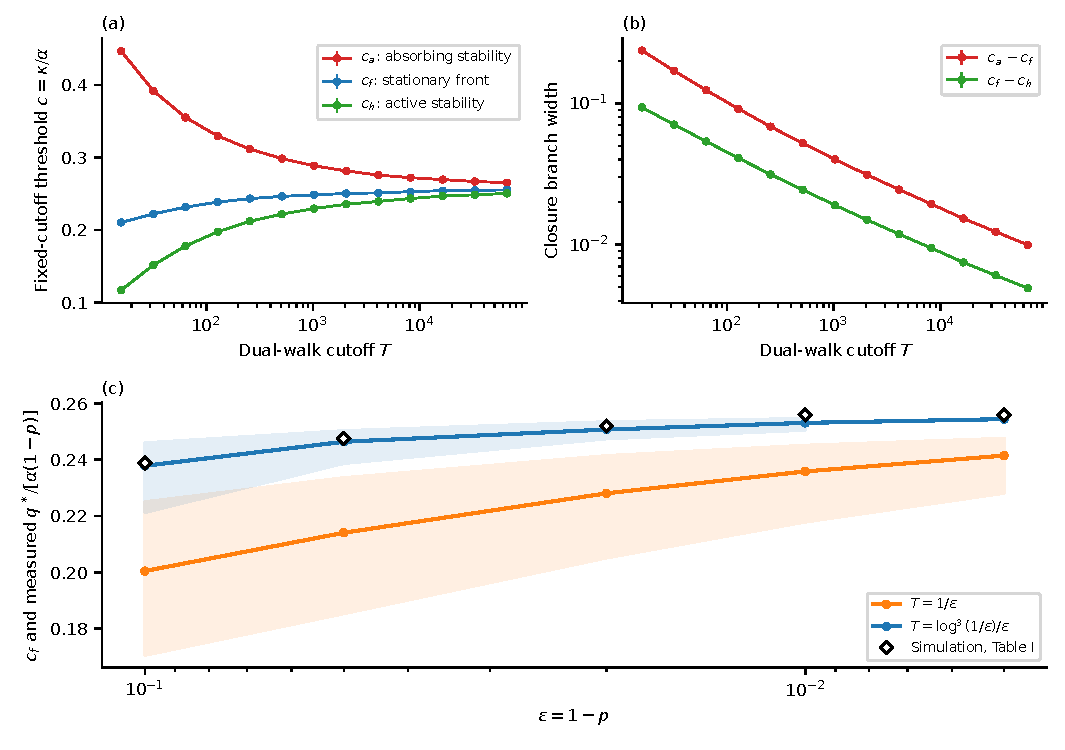
\includegraphics[width=\textwidth]{figs/fig_theory_v2}
\caption{Finite-time voter closure and cutoff sensitivity.
(a) Absorbing-state, stationary-front, and active-state thresholds at fixed
dual-walk cutoff $T$. Error bars represent approximately $95\%$ pointwise
Monte Carlo intervals, not closure uncertainty.
(b) The two branches of the bistable interval, with the covariance between
thresholds retained.
(c) Two illustrative matching prescriptions, $T=1/\varepsilon$ and
$T=\log^3(1/\varepsilon)/\varepsilon$, compared with the transition-line
central values in Table~\ref{tab:line}. Shading shows the change when the
prescribed time is multiplied by $A\in[1/4,4]$; it is a sensitivity envelope,
not a confidence band. No extrapolation beyond the recorded cutoffs is made,
so the upper envelope of the logarithmic prescription is incomplete at the
smallest $\varepsilon$.}
\label{fig:theory}
\end{figure*}

\subsection{Matching uncertainty and the voter endpoint}

In two dimensions the probability of retaining several distinct voter lineages
decays logarithmically with time~\cite{cox2010,cox2025}. The scale on which a
perturbation acts can therefore differ from $1/\varepsilon$ by logarithmic
factors. For example, the two-dimensional scaling of Ref.~\cite{cox2025}
uses $\varepsilon_N=(\log N)^3/N$. That result does not derive a matching
time for the present synchronous automaton, especially close to cancellation
of its leading cubic drift, but it motivates checking sensitivity to such
factors.

Figure~\ref{fig:theory}(c) compares the unadjusted prescriptions
$T=1/\varepsilon$ and $T=\log^3(1/\varepsilon)/\varepsilon$:
\begin{center}
\begin{tabular}{cccc}
$p$ & measured $c$ & $c_f(1/\varepsilon)$ & $c_f(\log^3(1/\varepsilon)/\varepsilon)$\\
\hline
0.9 & 0.2388 & 0.2005 & 0.2379\\
0.95 & 0.2476 & 0.2141 & 0.2464\\
0.98 & 0.2520 & 0.2281 & 0.2507\\
0.99 & 0.2560 & 0.2359 & 0.2531\\
0.995 & 0.2560 & 0.2415 & 0.2545
\end{tabular}
\end{center}
The logarithmic prescription substantially improves this comparison without
adjusting its prefactor. This agreement is a diagnostic of the importance of
the matching scale, rather than a validation of that prescription.
Multiplying either prescribed time by $A=1/4,1,4$ displays the remaining
sensitivity. Interpolation is linear in $\log T$; points beyond the recorded
range are left unevaluated.

The walk statistics constrain the closure much more precisely than they fix
its relation to the lattice process. For example, over $1024\le T\le65536$,
$c_f$ moves from $0.24843$ to $0.25526$, while its one-standard-error sampling
uncertainty grows from $0.00119$ to $0.00191$. We therefore do not assign a
confidence interval to a $T\to\infty$ amplitude. The same walks contribute
to successive checkpoint histograms; the stored marginal counts do not
recover their cross-time covariance, and we do not treat those checkpoints
as independent observations in an extrapolation.

The lazy-walk calculation gives another independent test of the closure.
At physical dual time $rT=65536$, it gives $c_f=0.2212$, $0.2060$, and
$0.2003$ for $r=1/2,1/4,1/8$, respectively, compared with measured values
about $0.218,0.216,0.219$. It captures the initial direction of the shift.
The measured differences among the smaller $r$ values lie below the
front-fit systematic variation discussed in Sec.~\ref{sec:async}, so this
comparison does not resolve a limiting amplitude. The five-cell rule in
Appendix~\ref{app:molofsky} supplies a sharper limitation: no single cutoff
reproduces its two stability boundaries and its front reversal.

The exact identities identify a mechanism available to a voter perturbation:
higher-lineage correlations generate the noncubic drift needed for a bistable
reaction term. They also explain why that contribution becomes small at long
voter times within the closure. Whether it remains effective after matching
and fluctuation corrections is not determined by the calculation. Persistence
of a first-order line for every fixed $p<1$, and its logarithmic approach to
the voter point, remain conjectures; the numerical evidence for finite $p$
is assessed separately in Sec.~\ref{sec:voter}.

\section{Discussion}
\label{sec:discussion}

The simulations support a discontinuous active--absorbing transition in a two-dimensional
binary model with exactly two symmetry-related absorbing configurations. At $p=1/2$, the
front reversal occurs while the active phase retains a finite interface density.
The active phase retreats as a coherent region, and bulk runs on its metastable side
decay through the growth of absorbing domains. Large droplets of the competing phases
exchange growth and shrinkage across the same narrow parameter range.
Small orientation-dependent crossing differences and temporal shifts are
resolved separately; an asymptotic interval of generic coexistence
remains unresolved~\cite{wang2015,liu2018}.
Together these measurements identify phase competition through independently measured
bulk and interfacial observables.

This result extends the two-dimensional picture of GV criticality and
Ising--DP splitting~\cite{dornic2001,droz2003,alhammal2005}. Earlier reports of discontinuous
behavior in two-state models~\cite{rodrigues2015} make the distinction between activity and
magnetization essential. The contribution here is the combined evidence for coexistence
in a model whose absorbing configurations are explicitly characterized.
The front phenomenology has close analogues in defensive-alliance
models~\cite{szabo2004,guisoni2013}; realizing it with binary sites and only two absorbing
configurations isolates the transition from internal dynamics within an absorbing phase.

A physical interpretation is competition between active and absorbing regions,
with front propagation opposed by curvature. On the side where an absorbing domain
invades, a sufficiently large fluctuation can initiate decay of the active phase.
On the other side, small absorbing domains contract.
A predictive theory would need to derive the front mobility, curvature response,
and nucleation rate from the microscopic rule. A local deterministic potential and
its noise amplitude alone do not determine those spatial quantities.

The continuation toward the voter point introduces a separate scale problem.
A small density jump, slow continuous vanishing, and a long crossover can be difficult
to distinguish over finite times. Nonlinear GV models can also have transient
magnetization drift and seed dynamics that differ from the linear voter
model~\cite{castellano2012,azizi2020}. Effective exponents therefore support the
interpretation together with independent boundary estimates and bulk and front
measurements with explicit time- and size-window checks. The asymptotic
endpoint remains an open question.

The coalescing-walk closure organizes the microscopic perturbations and accounts
approximately for the scale $q^*\sim\alpha(1-p)$. Higher-lineage contributions supply
terms capable of bistability within the closure, and their decreasing weight suggests
a narrowing bistable region. Establishing its asymptotic width requires a controlled
matching scale and the fluctuations beyond the local reaction term. Connecting this
construction to rigorous two-dimensional perturbation limits~\cite{cox2010,cox2025}
remains open.

The five-cell comparison makes the limitation concrete. The closure places the invasion
boundary close to simulation, but no single matching time describes that boundary and
all of its predicted stability limits. In particular, simulations do not resolve its
predicted metastable active branch. Small-seed suppression and a finite-time droplet
threshold characterize invasion dynamics; they do not alone settle the limiting order
of the transition. Understanding why the Day \& Night construction supports the
stronger coexistence signatures is a target for a theory of nonlinear voter rules.

A systematic weak-noise study of the spatial Langevin equation would test which
continuum parameters reproduce the observed coexistence. A controlled approach to the
voter endpoint could then establish whether the discontinuity survives arbitrarily
close to it or terminates before it.

\begin{acknowledgments}
Simulations were run on the Torch cluster at New York University.
\end{acknowledgments}

\section*{Data availability}
The simulator (Appendix~\ref{app:numerics}), parameter and seed manifests,
independent-run outputs, analysis scripts, and figure sources accompany this study.
The numerical analyses retain input hashes and per-run measurements so that the
figures and statistical summaries can be reproduced from the recorded data.

%=====================================================================================
\appendix

\section{Frozen configurations at $p = 0$}
\label{app:frozen}

At $p = 0$ the flip table is $w(j) = \alpha R(j) + q\,\delta_{j,2}$, so every configuration in
which all sites have $j\in\{0,1,4,5\}$ is frozen. A local construction proves
that their number grows exponentially with area. Start from a checkerboard
on a torus whose lengths are divisible by four. Independently choose whether
to complement each $2\times2$ block with lower-left corner $(4a,4b)$.
For one complemented block, its four sites and the four exterior diagonal
corners have $j=5$; the other sites in its surrounding $4\times4$ square
retain $j=4$. The affected neighborhoods of different blocks are disjoint,
so every choice is frozen. Hence, with $N=L_xL_y$,
\begin{equation}
 \mathcal N_{\rm frozen}\ge 2^{N/16},\qquad
 \frac{\ln\mathcal N_{\rm frozen}}{N}\ge\frac{\ln2}{16}.
 \label{eq:frozenbound}
\end{equation}
This bound holds for every admissible $q$ at $p=0$.

Transfer-matrix counts on periodic strips of fixed widths $W=7$ and $8$
give a larger strip entropy, $\mathcal N_W\sim e^{s_WN}$ with
$s_W\approx0.32$ per site, against $\ln2\simeq0.69$ for all configurations.
These two strip widths do not determine the two-dimensional entropy density.
As a check,
on the $3\times3$ torus, where every site neighbors every other, the count is
$254 = 1 + \binom94 + \binom95 + 1$. The simplest examples are the two checkerboards and the
diagonal stripes of width two, in which every site has $j = 4$.

These exceptional configurations did not attract the tested random starts at $q>0$. Random initial conditions at $L = 256$
run to $t = 10^6$ at $q = 0.005$--$0.018$ (all below $\qs$) end in one of the two uniform states.
In the active phase ($q = 0.03$--$1$) the frequency of locally checkerboard or stripe-like
$3\times3$ blocks stays at the level expected by chance. A prepared half-lattice of either pattern
next to an active or a dead half is eroded completely within $10^4$ steps at every $q$ tested,
including $q = 0$, and a single flipped site destroys a perfect $256\times256$ pattern within
$\approx 10^3$ steps (in 11 of 12 runs). Only at $q = 0$, where $j = 2$ sites are also frozen, does
the dynamics stop with a small density ($\approx 1\%$) of frozen debris.

Removing the frozen configurations directly by a flip probability $\epsilon$ at
$j\in\{1,4,5\}$ preserves the linear reversal of the front velocity: at $\epsilon = 0.003$ the
velocity is $-0.0041$, $-0.0002$, $+0.0024$, $+0.0053$ at $q/\qs(0) = 0.88$, 0.92, 0.96, 1.00, so
$\qs(\epsilon)\approx 0.92\,\qs(0)$, and at $\epsilon = 0.01$, $\qs\approx 0.8\,\qs(0)$, with
an interior interface fraction 0.44--0.6 behind the front. These checks retain
front reversal and an active interior after removing the extra frozen states.
They suggest a smooth small-$\epsilon$ continuation over the measured range;
they do not establish the infinite-time $p\to0^+$ limit of the voter-admixed family.

\section{Pair approximation}
\label{app:pa}

We closed the dynamics at the level of nearest-neighbor pairs on a Bethe lattice with $z = 8$:
given a site's state, its neighbors are independent and disagree with it with probability
$\theta_s = \rho/(2x_s)$, where $\rho$ is the fraction of disagreeing bonds and $x_s$ the fraction
of sites in state $s$. Both the continuous-time version and the synchronous map were analyzed.
In the voter limit the continuous-time closure conserves $m$ and gives $\rho^*=(z-2)(1-m^2)/[2(z-1)]$. The synchronous map differs: at $m=0$ its active fixed point is $\rho^*=1/2$. For every
$p<1$ a dilute minority in an absorbing state decays at rate
$(1-p)\alpha P_R(\theta) + qP_2(\theta)$, where $\theta$ is the conditional
disagreement probability around a minority site,
$P_j(\theta)=\binom{8}{j}\theta^j(1-\theta)^{8-j}$, and
$P_R=P_3+P_6+P_7+P_8$. Thus the absorbing states are linearly stable in the
parameter range studied, and the
symmetric active fixed point ($\rho^*\approx 0.43$--$0.50$) is stable over the
parameter grid checked. The approximation is bistable over that grid and
does not select a coexistence point; a
front criterion based on it gets $\qs\propto(1-p)$ near the voter point but with an amplitude off
by a factor of two, and fails qualitatively for $p\lesssim 0.5$. This is why we rely on the
perturbation theory of Sec.~\ref{sec:theory}.

\section{A second rule: noise on the forbidden flips of D\&N}
\label{app:eta}

To check that the discontinuity does not depend on the voter admixture, we studied the rule
\begin{equation}
w(j) = \alpha R(j) + \eta\,[\,j\in\{1,2,4,5\}\,],
\label{eq:eta}
\end{equation}
in which every flip that D\&N forbids, except at $j = 0$, happens with a small probability $\eta$.
For $0<\alpha,\eta\le1$, the lemma of Sec.~\ref{sec:lemma} gives exactly
two absorbing states. At $\alpha = 1/2$, strip
fronts ($L_x = 2048$, $L_y = 4096$, $T = 10^5$, three seeds) retreat at $v = -0.0022\pm0.0010$ for
$\eta = 0.01275$ and advance at $v = +0.0020\pm0.0001$ and $+0.0054\pm0.0001$ for $\eta = 0.013125$
and $0.01375$, so $\eta^*\approx 0.0130$ (linear interpolation: $0.01295$). Bulk runs at $L = 1024$ and 2048 (two seeds each,
$T = 2\times10^5$) have last-half interface densities
$\rho\simeq0.25$ at $\eta = 0.013125$ ($\approx
1.01\,\eta^*$) and $\rho\simeq0.276$ at $0.01375$, at both sizes. Below $\eta^*$ the prepared active phase decays: at $\eta = 0.01275$ it decays slowly (from $\rho = 0.236$ at $t = 10^4$ to $0.17$ at
$2\times10^5$), and at $\eta = 0.0125$, $0.01225$, $0.011875$, and $0.01125$ its half-life is
$(5.3$--$6.4)\times10^4$, $(2.6$--$3.2)\times10^4$, $(1.3$--$1.6)\times10^4$, and $(0.8$--$0.9)
\times10^4$, similar at the two sampled sizes. Here the half-life is the first
recorded crossing below half the density at $t=10^3$, rather than consensus.
Together these finite-window front and bulk checks support a discontinuity
with an active-side density of order 0.25 in this second rule
(Fig.~\ref{fig:eta}).

\begin{figure}
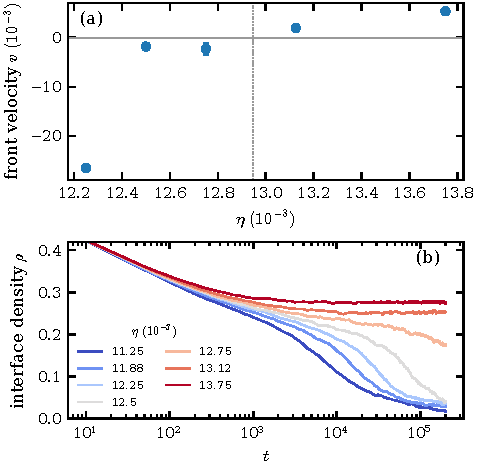
\includegraphics[width=\columnwidth]{figs/fig_eta}
\caption{The rule of Eq.~\eqref{eq:eta} at $\alpha = 1/2$. (a) Strip-front velocity against $\eta$
(three runs per $\eta$; plotted means retain fits with at least 20 records,
including only two runs at $\eta=0.01225$). The strongly negative
$\eta=0.01225$ estimate uses a short window before the strip interior orders;
it is not a late planar-front velocity. The dotted line is
$\eta^*=0.01295$. (b) Example bulk trajectories (seed 1) at $L=2048$.}
\label{fig:eta}
\end{figure}

\section{The five-cell rule of Molofsky \emph{et al.}: closure and simulation}
\label{app:molofsky}

\textit{Rule and closure.} The rule of Ref.~\cite{molofsky1999} is synchronous on the square
lattice, and a site's next state depends on the number $n$ of species-1 cells among the five
cells of its von Neumann neighborhood including itself: it becomes 1 with probability $p_n$,
where $p_0 = 0$, $p_5 = 1$, $p_3 = 1-p_2$, and $p_4 = 1-p_1$. In terms of the number $j$ of
disagreeing neighbors among the four, both states flip with probability $w(j) = p_j$.
For the interior parameters $0<p_1,p_2<1$ studied near the voter point, every
nonuniform configuration has a site with positive flip probability, so the two
uniform states are the only absorbing configurations. The rule is
$\mathbb{Z}_2$-symmetric, and its voter point is
$(p_1,p_2) = (1/5,2/5)$, where $w(j) = j/5$: the site copies one of the five cells, itself
included. Writing $w(j) = j/5 + g(j)$ gives $g = (0,\delta_1,\delta_2,-\delta_2,-\delta_1)$ with
$\delta_1 = p_1 - 1/5$ and $\delta_2 = p_2 - 2/5$. The dual of the voter point is a system of
five lazy coalescing walks, started at a site and its four neighbors, each staying with
probability $1/5$ or stepping to a neighbor with probability $1/5$; we sampled their lineage
patterns ($10^7$ samples per $T$) and evaluated the reaction function as in
Sec.~\ref{sec:theory}. Its structure is simpler than for the Moore neighborhood: with
$h(u) = u(1-u)(1-2u)$,
\begin{equation}
f(u) = h(u)\,[\,a + c\,u(1-u)\,],
\label{eq:fmol}
\end{equation}
with $a = \delta_1 a_1 + \delta_2 a_2$ and $c = P_5\,(10\,\delta_2 - 5\,\delta_1)$, where
$P_5(T)$ is the probability that all five lineages are distinct (the only five-class pattern,
which contributes exactly the mean-field map of Ref.~\cite{molofsky1999}) and $a_1$, $a_2$
collect the linear coefficients from all patterns, including the five-lineage
pattern. Then $f'(0) = a$, $f'(1/2) = -(a + c/4)/2$, and
$\int_0^{1/2} f\,\ds u = (6a+c)/192$. Both $u = 0$ and $u = 1/2$ are stable, with the front
reversing in between, in the sector $-c/4 < a < 0$ of the $(\delta_1,\delta_2)$ plane, whose
angular width is set by $P_5$. At fixed $c>0$, the front reversal $a=-c/6$
lies two thirds of the way from $a=0$ to $a=-c/4$ in coefficient space;
this fraction need not be the same in the angular coordinate of the microscopic
parameters. This two-parameter rule accesses a bistable sector at finite $T$.
Whether a one-parameter family crosses such a sector depends on its path through
coefficient space, as well as on the higher-lineage weight.

Table~\ref{tab:molofsky} and Fig.~\ref{fig:molofsky}(a,b) give the closure's result. The sector
lies in the direction of small $p_1$ and large $p_2$, inside the mean-field multiple-outcome
wedge, around a line through the voter point of slope $\ds p_2/\ds p_1 = -3.46$ at $T = 65536$;
the empirical clustering--ergodic boundary of Ref.~\cite{molofsky1999}, which passes through
$(0.024, 1)$ and is described there by the dyad rule $3p_1 + p_2 = 1$, has slope $-3.4$ to $-3$
through the voter point. The window is $4.4^\circ$ wide at $T = 16$ and $0.45^\circ$ at
$T = 1024$, four to eight times narrower in relative terms than the D\&N window at the same $T$,
because five walks started on a plus stay distinct ten to forty times more rarely than nine
started on a $3\times3$ block. At the matching distance $\rho = 1/T$ from the voter point it is
about $5\times10^{-3}$ wide in $p$ at $T = 16$ and $5\times10^{-4}$ at $T = 64$.
These widths depend on the illustrative matching prescription. Ref.~\cite{molofsky1999}
used both small seeds and random-density initial conditions, but did not resolve
the multiple outcomes predicted by mean field. The narrow closure sector suggests
a reason for further tests; it does not establish that a metastable spatial branch exists.

\begin{table}
\caption{The closure for the five-cell rule of Ref.~\cite{molofsky1999}: fraction of five-class
patterns among those with at least three classes, directions (degrees from the $+\delta_1$ axis)
of the rays $f'(0) = 0$ ($\theta_a$), $\int_0^{1/2} f = 0$ ($\theta_{\rm front}$), and
$f'(1/2) = 0$ ($\theta_{1/2}$), and the angular width of the bistable sector; $10^7$ samples per
$T$, bootstrap errors $\le 0.05^\circ$. Mean field ($T = 0$): $90^\circ$, $111.8^\circ$,
$123.7^\circ$, width $33.7^\circ$.}
\label{tab:molofsky}
\begin{ruledtabular}
\begin{tabular}{llllll}
$T$ & $P_5/P_{\ge3}$ & $\theta_a$ & $\theta_{\rm front}$ & $\theta_{1/2}$ & width \\
\hline
16 & 0.066 & 104.34 & 107.28 & 108.77 & 4.43 \\
64 & 0.025 & 105.32 & 106.60 & 107.25 & 1.92 \\
256 & 0.011 & 105.73 & 106.32 & 106.62 & 0.90 \\
1024 & 0.0052 & 105.93 & 106.23 & 106.38 & 0.45 \\
4096 & 0.0027 & 106.03 & 106.19 & 106.27 & 0.24 \\
65536 & 0.0008 & 106.09 & 106.14 & 106.17 & 0.07 \\
\end{tabular}
\end{ruledtabular}
\end{table}

\textit{Simulation.} We therefore simulated the rule itself, with the von Neumann neighborhood
added to the code of Appendix~\ref{app:numerics}, along two cuts across the predicted line,
$p_2 = 0.45$ and $0.50$, at distances $0.052$ and $0.104$ from the voter point. The protocol is
that of Sec.~\ref{sec:flagship}: planar fronts from a strip of the active phase ($L_x = 1024$--4096,
$L_y = 4096$, $6\times10^4$--$10^5$ steps, two to eight seeds, steps of $2.5\times10^{-4}$ in
$p_1$ near the reversal and of $10^{-4}$, down to $0.5\times10^{-4}$, within $3\times10^{-4}$ of
it), the mean population of $2\times2$ seeds (up to $2\times10^4$ replicas, $10^4$
steps), active disks of radius $R$ in the absorbing state (up to 400 replicas, $2\times10^4$
steps), and bulk runs from random initial conditions ($L = 256$--4096, $6\times10^4$--$1.2\times10^6$
steps, eight seeds at $L = 2048$ within $3\times10^{-4}$ of the line). At the voter point the mean population of a seed is conserved and the interface density
decays as $1/\ln t$, and at the three points on the edge $p_2 = 0$ described in
Ref.~\cite{molofsky1999} we reproduce their invasion, phase separation, and clustering.
Table~\ref{tab:molsim} and Fig.~\ref{fig:molofsky}(c) summarize the rest.

\begin{table}
\caption{Simulation of the five-cell rule of Ref.~\cite{molofsky1999} on the cuts $p_2 = 0.45$
and $0.50$ across the predicted line (distances $0.052$ and $0.104$ from the voter point),
against the closure of Table~\ref{tab:molofsky}. Directions are in degrees from the $+\delta_1$
axis; $p_1^*$ is the front reversal and $\Delta p_1 = p_1 - p_1^*$; ``seeds decay'' means that the mean population of a
$2\times2$ seed decreases over the first $10^2$--$10^3$ steps;
$R_{1/2}$ is the finite-time half-survival radius at $2\times10^4$ steps.
Disk ensembles stop at 100 terminal survivors or 400 replicas per radius;
all escape counts are zero. These adaptive estimates are descriptive.
$\rho$ is the interface density of the active phase. The boundary of observed bulk stationarity lies
between the reversal and $0.5\times10^{-4}$ above it. The corresponding
$\theta_{\rm stat}$ is a finite-window estimate, not a measured linear-stability
limit; the closure comparison uses its active-state stability threshold.}
\label{tab:molsim}
\begin{ruledtabular}
\begin{tabular}{lll}
 & $p_2 = 0.45$ & $p_2 = 0.50$ \\
\hline
$p_1^*$ & $0.18535(3)$ & $0.17057(3)$ \\
$\theta_{\rm front}$ & $106.33$ & $106.40$ \\
\quad closure, $T = 16$, $1024$, $65536$ & \multicolumn{2}{l}{$107.28$, $106.23$, $106.14$} \\
seeds decay for $\Delta p_1 <$ & $1.7\times10^{-3}$ & $2.4\times10^{-3}$ \\
\quad i.e. $\theta_a\approx$ & $104.5$ & $105.0$ \\
\quad closure, $T = 16$, $64$, $1024$ & \multicolumn{2}{l}{$104.34$, $105.32$, $105.93$} \\
$R_{1/2}v$ & $0.18$ & $0.16$--$0.19$ \\
bulk stationary for $\Delta p_1\ge$ & $0.5\times10^{-4}$ & $0.5\times10^{-4}$ \\
\quad not stationary for $\Delta p_1\le$ & $0.4\times10^{-4}$ & $0$ \\
\quad i.e. $|\theta_{\rm stat} - \theta_{\rm front}|\le$ & $0.05$ & $0.03$ \\
\quad closure, $T = 16$, $64$, $1024$ & \multicolumn{2}{l}{$1.49$, $0.65$, $0.15$} \\
$\rho$ at $\Delta p_1 = 0.5\times10^{-4}$ & $0.188(1)$ & $0.20$ \\
$\rho$ at $\Delta p_1 = 1.5\times10^{-4}$ & $0.210(1)$ & $0.22$ \\
\end{tabular}
\end{ruledtabular}
\end{table}

\begin{figure}
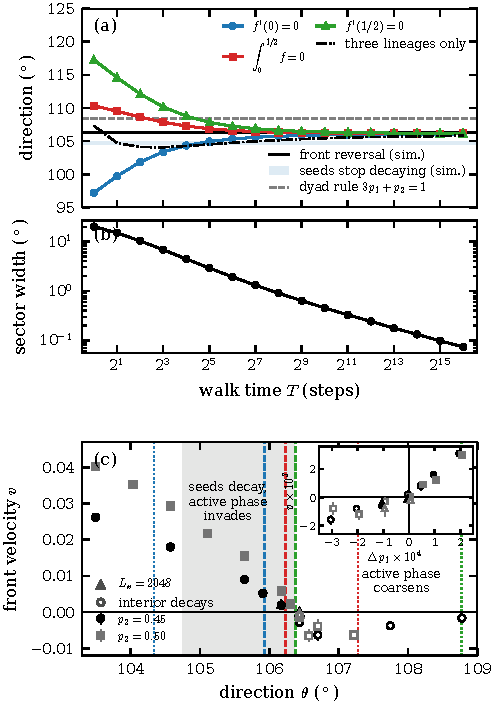
\includegraphics[width=\columnwidth]{figs/fig_molofsky}
\caption{The five-cell rule of Molofsky \emph{et al.}~\cite{molofsky1999}
(Appendix~\ref{app:molofsky}). (a) The closure: directions, in the plane $(\delta_1,\delta_2) =
(p_1-1/5,\,p_2-2/5)$ around the voter point, of the rays on which the absorbing state loses
linear stability, the front between the absorbing and the active state is stationary, and the
active state loses stability, against the walk time $T$; the bistable sector lies between the
first and the third. Solid line: the front reversal found by simulation,
$106.33^\circ$--$106.40^\circ$, which is also the direction of the chord from the voter point to
the boundary point $(0.024, 1)$ of Ref.~\cite{molofsky1999}; dashed line: their dyad rule
$3p_1+p_2 = 1$; band: where the mean population of a $2\times2$ seed stops decreasing in the
simulation. (b) Angular width of the sector. (c) The simulation: velocity of a planar front
(rows per step, positive when the active phase invades) against the direction $\theta$ on the
cuts $p_2 = 0.45$ (circles) and $0.50$ (squares); open symbols, the interior of the strip decays
during the run; triangles, $L_x = 2048$. Vertical lines: the closure's rays at $T = 16$ (dotted)
and $1024$ (dashed), colored as in (a). Shaded: the band in which small seeds initially
decline while a prepared active phase invades. Inset: the crossing at steps of $10^{-4}$ in $p_1$
($L_x = 2048$ and, triangles, 4096; $L_y = 4096$, $10^5$ steps), against $\Delta p_1 = p_1 -
p_1^*$; the interior of the strip is stationary over the run (filled symbols) wherever $v > 0$
and decays (open) wherever $v\le0$.}
\label{fig:molofsky}
\end{figure}

The closure approximately locates the invasion line. The front velocity is linear in $p_1$ through zero, with
slope $14$--$15$ at the reversal, at $p_1^* = 0.18535(3)$ and $0.17057(3)$ on the two cuts, the
error being the spread between three estimators of the velocity at $L_x = 2048$ and 4096. The
two reversals and the voter point are collinear, at $106.33^\circ$ and $106.40^\circ$ from the
$+\delta_1$ axis, slope $\ds p_2/\ds p_1 = -3.41(1)$ against the closure's $-3.46$;
extended, the line meets $p_2 = 1$ at $p_1 = 0.0235$, where Ref.~\cite{molofsky1999} places its
boundary point $(0.024, 1)$, and $p_2 = 0$ at $p_1 = 0.318$, between their phase separation at
$0.31$ and their invasion at $0.35$.

On the side where the active phase invades, small-seed and large-droplet dynamics
differ markedly. In the recorded finite-time samples, the mean population
of a $2\times2$ seed decreases for $p_1$ up to $1.5$--$2.5\times10^{-3}$ above $p_1^*$, i.e. up
to $\theta_a\approx 104.5^\circ$--$105^\circ$, as the closure gives for $T\approx 16$--$64$, the
terminal survival at $10^4$ steps is rare: for example, only 93 of
20\,000 seeds survive at $(p_2,p_1)=(0.45,0.186)$.
For active disks, survival to $2\times10^4$ steps crosses one half at a
radius $R_{1/2}$ in four parameter sets, with
$R_{1/2}v=0.1595$--$0.1846$, close to $D=1/5$, the diffusion constant of
the lazy walk. A fifth set gives only $R_{1/2}>28$ over the sampled radii.
No boundary escapes occurred in either experiment, so survival at the stated
horizon is observed directly. These ensembles used adaptive stopping:
disks stopped at 100 terminal survivors or 400 replicas, and small seeds at
300 survivors or 20\,000 replicas. We therefore treat these estimates
descriptively; they do not determine an asymptotic critical radius.
The active phase is
stationary down to $0.5\times10^{-4}$ above $p_1^*$, where its interface density is $0.188(1)$
at $L = 2048$ and $0.190(1)$ at $L = 4096$. At $0.4\times10^{-4}$ it no longer settles, the
seeds wandering between $0.15$ and $0.19$ and $L = 4096$ drifting down to $0.176(3)$; at
$0.3\times10^{-4}$ it declines, and at $p_1^*$ it coarsens away. The density of the stationary
branch falls without a plateau from $0.30$ at $5\times10^{-3}$ above the line to $0.204(1)$ at
$10^{-4}$ and $0.188(1)$ at $0.5\times10^{-4}$, linearly in $\ln\Delta p_1$ at $0.021(5)$ per
$e$-fold, which $A/\ln(B/\Delta p_1)$, a power $\Delta p_1^{0.10}$, and a jump
$\rho_0 + C\,\Delta p_1^{0.3}$ with $\rho_0 = 0.14$ all reproduce with $p_1^*$ at the reversal
($\chi^2$ per degree of freedom $1.2$, $0.5$, $2.3$; a free $\rho_0$ stays below $0.12$ at two
standard deviations). But the tested continuous forms anchored there predict $0.18$ at the two points
below $0.5\times10^{-4}$, $0.01$--$0.03$ above what is measured, and with $p_1^*$ free every form
moves the line $1$--$4\times10^{-5}$ above the reversal, within its error and onto the edge of observed
stationarity. The fitted logarithmic form is compatible with these finite-window
data when the line is $1$--$4\times10^{-5}$ above the reversal's central value,
where the density $10^{-5}$ from
the line would still be $0.17$; telling that from a jump needs the line to better than
$10^{-5}$, and our data do not decide it. The band of suppressed initial seed growth is about $1.5^\circ$--$2^\circ$ wide. It resembles the invasion-versus-small-seed contrast of Case~4A in Ref.~\cite{cox2013}, but finite-time seed decay does not establish asymptotic linear stability. Its narrowness provides a possible explanation for why the earlier scan did not resolve such behavior.

Across the line the two sides differ. No metastable active branch is resolved by these runs. At the
reversal and $1$--$3\times10^{-4}$ below it, its interface density declines from the start, only
slightly faster than the voter model's own $1/\ln t$, and the time to absorption grows with $L$,
by a factor $1.5$--$3.5$ from $L = 256$ to 512 (from $0.5$--$1.4\times10^5$ to
$1.1$--$2.0\times10^5$ steps below the line, and from $2.3$--$2.4\times10^5$ to
$4.6$--$8\times10^5$ at $p_1^*$ itself), as domains coarsen to the system size; the metastable
active phase of D\&N instead decays by nucleation after a plateau, with its
half-density decay time approaching an $L$-independent value over the largest
sampled sizes [Fig.~\ref{fig:bulk}(c)]. Nowhere below the reversal does a stationary active slab
retreat: where $v < 0$ the strip dissolves in place, its interior at half of its early density
by $10^5$ steps already $10^{-4}$ below $p_1^*$, and wherever the interior is stationary,
$v > 0$ [Fig.~\ref{fig:molofsky}(c), inset]. Observed bulk stationarity is thus lost within
$0.5\times10^{-4}$ of the reversal, i.e. within $0.05^\circ$ and $0.03^\circ$ on the two cuts,
and on the invading side of it if anywhere, where the closure puts the ray $f'(1/2) = 0$ beyond
the front by $1.5^\circ$ at $T = 16$, $0.65^\circ$ at $T = 64$, and $0.15^\circ$ at $T = 1024$.
The two protocols therefore reveal a marked asymmetry: small seeds are suppressed where a macroscopic active region invades, while no stationary retreating active slab is resolved. Since the density data do not determine the limiting jump, we leave the order of this transition open. The closure locates the line to $0.3^\circ$
and approximately locates the initial seed-suppression crossover at suitable
matching times. Its predicted active-state stability range extends beyond
the observed stationarity range at every $T$ we computed; no
single $T$ fits the three rays, since $\theta_a$ wants $T\approx 16$--$64$, the natural
$T\sim 1/\rho$, the front is matched at $T\approx 300$, and the bound on $\theta_{1/2}$ needs
$T\gtrsim 10^4$. The caveats of Sec.~\ref{sec:theory} apply. Why the active-state branch is wide for D\&N, whose active phase is
metastable down to $0.9\,\qs$, and absent here, the closure does not explain; its
fixed-cutoff form~\eqref{eq:fmol} does not reproduce the observed separation of
invasion and relaxation scales with one matching time.
\section{Numerical details}
\label{app:numerics}

\textit{Code.} The simulator stores 64 sites per 64-bit word. The eight neighbor bits of all sites
of a word are summed with bitwise adder trees, giving the number of live neighbors $k$ in four
bit planes; the flip class of each site is $(\sigma, k)$, with the flip probability $f_{\sigma k}$
read from an $2\times 9$ table, so that any outer-totalistic rule, Eq.~\eqref{eq:rule}, and the lazy
tables of Sec.~\ref{sec:async} are run by the same kernel. Each site draws one 32-bit uniform per
step from Philox$4\times32$-10~\cite{salmon2011} with counter (time, row, word, draw), and the 64
comparisons with the per-class thresholds are done bit-serially in parallel. Validation: (i) a
bit-exact comparison with a naive per-site implementation for five rules on four lattice shapes,
including one-word-wide and three-row lattices; (ii) per-class flip frequencies for an 18-class
table (variance of the $z$ scores over 560 repetitions $1.04\pm0.06$) and a $1.3\times10^8$-sample
test of the shared comparison on a voter-like table (per-class frequencies and adjacent-lane
independence, $|z|<2$); (iii) identical output for any number of threads and across restarts
from checkpoints; (iv) agreement with an independent GPU implementation of the $p = 0$ model to
1\% in the stationary density.

\textit{CUDA extension.} The dense GPU backend uses the original CPU integer
flip function and Philox implementation, extracted automatically into device
code. Two lattice buffers implement simultaneous updates; batches of 256 steps
are submitted as CUDA graphs without changing the update order or counters.
The host retains initialization, observables, profiles, and checkpoint format.
Validation compares full configurations, time series, profiles, snapshots, and
checkpoints byte for byte with the CPU implementation. Cases include one-word
rows, an $L=2048$ lattice, Moore and von Neumann neighborhoods, lazy update
tables, irregular output schedules, graph-batch boundaries, and counters near
$2^{32}$. CPU-to-GPU and GPU-to-CPU restarts reproduce the same trajectories.
The GPU checks absorption at scheduled outputs, so its absorption times are
interval observed. The lifetime and sparse-replica campaigns use the CPU code.
Parameter manifests record distinct 64-bit seeds, source and executable hashes,
and completion status; interrupted runs are identified rather than silently
pooled with completed ensembles.

\textit{Replica mode.} For seeds and droplets, only the bounding box of the sites with a
disagreeing neighbor (plus a margin) is updated, refitted every 32 steps. This is exact because a
site with $j = 0$ cannot flip and its random numbers are indexed by position, not by the order
of updates; over 200 seeds, box and full-lattice updating give identical configurations at
every step. A replica whose box comes within 2 rows or 64 columns of the lattice edge is stopped
and recorded as an escape. Its later survival is unobserved; the
seed-curve convention retains it as a separately tabulated contribution,
while the droplet growth observable counts the escape itself. In the pure voter model the method reproduces the martingale
$\langle A(t)\rangle = 4$ for the number of live sites of a $2\times2$ seed (within $|z|<0.94$
at all 38 output times over $2\times10^5$ replicas) and $P_s(t)\propto\ln t/t$.

\textit{Front tracking.} The broad strip survey in Table~\ref{tab:line}
uses a smoothed row profile and local interpolation of the velocities bracketing
reversal. For the orientation, extended-strip, and $p=1/2$ lazy-update
analyses, we explicitly track
the outer envelope: the lowest and highest bins whose smoothed activity exceeds
$0.3$ of the interior reference value measured at $t=10^3$. An interior hole
cannot stop this envelope. We also retain the center-connected-component width,
interior activity, and hole fraction as diagnostics. No run is removed simply
because its interior density is small in these corrected analyses.
The other supporting parameter surveys retain their legacy center-connected
tracker and interior-activity validity criterion; their crossing estimates
are not assigned the precision of the extended campaign.

For a tilted band, $s=(ay-bx)\bmod L$ has $L$ bins containing $L$ sites each,
with normal spacing $1/\sqrt{a^2+b^2}$. Smoothing is over nine normal lattice
spacings, converted to an odd number of bins. The front speed is half the slope
of the normal width. Fits stop when the band leaves the width range
$[0.15L,0.85L]$ in bin coordinates, before winding or disappearance invalidates
the geometry. In the broad orientation survey the principal window begins at
$t=2\times10^4$; fits starting at $10^4$ and $4\times10^4$ and threshold
fractions 0.2, 0.3, and 0.5 quantify sensitivity. Local bracketing estimates,
linear fits over wider intervals, and quadratic fits are compared explicitly.
Independent runs are resampled within each $q$ for the crossing intervals;
uncertainty from the fit model or time window is reported separately. The
extended campaign additionally compares late and nonoverlapping time windows;
each published fit requires full coverage of its declared window for every seed.

\textit{Sampling uncertainty.} Independent realizations are the statistical
units; lattice sites and successive output records are not treated as
independent samples. For scalar means and paired mean differences in the new
four-run ensembles, percentile intervals enumerate all $4^4=256$ ordered
empirical bootstrap resamples. This removes Monte Carlo error in the
resampling calculation, not the limited coverage accuracy from four runs.
Front-crossing intervals additionally condition on the stated interpolation,
window, and geometrical eligibility. Pointwise intervals are distinguished
from the simultaneous orientation contrasts. Exact binomial intervals are
used for fixed-count survival endpoints. All these sampling intervals remain
separate from finite-size, finite-time, and estimator sensitivity.

\textit{Spatial correlations.} The large-system correlations are evaluated
directly from the final packed-bit configurations, using periodic shifts in
each coordinate direction. Each stored configuration is checked against its
recorded size, time, digest, magnetization, and nearest-neighbor activity;
the identity $C(1)=1-2\rho$ supplies an additional consistency check.
All declared runs are retained. The same resampled run indices are used at
every separation when constructing the pointwise uncertainty bands.
These final-time measurements do not assume an exponential correlation form.

\textit{Droplets and holes.} In the two-droplet test (Sec.~\ref{sec:fronts}) the dead hole is cut
into a lattice that is random at $t = 0$ and relaxes to the active phase within $10^3$ steps. Since
the active phase has alive density $1/2$ by symmetry, the hole's chord in row $y$ is $L_x$ minus
twice the number of live sites in that row, and its area is the sum of the chords; the active
disk's area is twice its number of live sites. The radius $R = (A/\pi)^{1/2}$ is fitted for
$t\ge 10^4$.

\textit{Layer edges.} For the roughness of the wetting layer (Sec.~\ref{sec:wall}) full
configurations were stored every $10^5$ steps. In each column the two edges of the layer are its
lowest and highest interface sites within $L_y/4$ of the wall; their variances along the wall and
the height-difference correlation $\langle[h(x+r)-h(x)]^2\rangle$ give the roughness.

\textit{Cost.} The earlier CPU campaigns used approximately 2200 core hours,
on Intel Xeon Platinum 8592+ nodes and a workstation, at
$(0.9$--$2.8)\times10^9$ site updates per second per core. The additional
campaign used 58.4 GPU allocation hours on NVIDIA H200 devices and
99.0 CPU-only allocated core hours. These allocation totals include validation,
I/O, and failed or restarted attempts; GPU-host CPU allocations are recorded
separately. Across the 40 staged GPU workers, mean sampled utilization during
simulation runs ranged from 92.7\% to 99.9\%. These samples include in-run
I/O but exclude build, validation, inter-task staging, and each run's initial
20 seconds; they are not allocation-wide efficiency estimates.

\bibliography{refs}

\end{document}
